%!TEX root = ../thesis.tex
%*******************************************************************************
%****************************** Second Chapter **********************************
%*******************************************************************************
\chapter{LAG SIM: A versatile, user-friendly structured illumination microscope} \label{chap:LAGSIM}

% Don't forget to PEE/L! 

% Note, figure labels are a bit of a mess here and need some fairly serious cleaning up! 04/10/18

% **************************** Define Graphics Path **************************
\ifpdf
    \graphicspath{{Chapter2/Figs/Raster/}{Chapter2/Figs/PDF/}{Chapter2/Figs/}}
\else
    \graphicspath{{Chapter2/Figs/Vector/}{Chapter2/Figs/}}
\fi

``The LAG SIM works good now and I really love it!''

\textit{Email from Meng Lu (Molecular Neuroscience Group, Cambridge), 26-06-2018}

\section{Introduction} \label{sec:simintro}
\subsection{Background}
Epifluorescent, widefield microscopy use a field of light to illuminate a labelled sample. 
Floresecnet emmission light is then emitted from any fluorescent molecule located within the microscope's field of view. 
Fluorescent molecules above and below the focal plane of the lens will also receive illumination light and fluoresce, causing an out-of-focus blur on the image with intensity [$\frac{1}{z^2}$ ??] where $z$ is axial distance from the focal plane. 

Out-of-focus light can be removed by lacing a pinhole in the excitation and emission path, and scanning the small spot of light across the sample to build up an image one pixel at a time. 
This technique, invented in 1955 and called confocal microscopy, physically blocks out-of-focus light, making 3D reconstructions of samples possible. 
The cost of this optical sectioning is a slow acquisition speed due to the nature of a point-scanning technique. 

A faster way of removing out-of-focus light can be achieved with total internal reflection fluorescence (TIRF). 
In this scheme light is projected into the outer edge of the back-aperture of a specialised lens, such that it emerges from the lens steeper than the critical angle required for reflection, rather than refraction, from a glass interface. 
Although this means that no light passes above the microscope slide, energy from the evanescent is able to couple into molecules close to the coverglass, inducing fluorescence. 
TIRF illuminates molecules within \SI{100}{\nano\metre} of the coverglass without being obscured by out-of-focus light, with the disadvantage that details deeper into the sample cannot be observed. % probably swap these two paragraphs: TIRF then OS

Sheppard [1990 + others] and Wilson [1984, 1997] showed that optical sectioning can be achieved computationally if the illumination light is modulated with a structured pattern. 
Illuminating the sample through a grating to produce a 2D sinusoidal illumination pattern, and moving the pattern through 3 evenly-spaced phase steps, produces 3 images described by Equation~\ref{eq:wilson-illumination}, where $i=\left\lbrace1,2,3\right\rbrace$ for three phase steps, $W$ is the sample fluorescence produced by a widefield image, $m$ the modulation index, $t$ the modulation frequency, $x$ a lateral spatial dimension in the sample plane, and $phi_i = \left\lbrace0, \frac{2\pi}{3}, \frac{4\pi}{3}\right\rbrace$ the phase steps of the illumination pattern. 

\begin{equation} \label{eq:wilson-illumination}
I_i = W \left( 1 + m \cos \left(t x + \phi_i \right) \right)
\end{equation}

To remove the out-of-focus unmodulated component from the reconstructed image $I_R$, we borrow from communication theory and use either square-law detection shown in Equation~\ref{eq:wilson-square-law}, or heterodyne detection shown in Equation~\ref{eq:wilson-heterodynne}. 

\begin{equation} \label{eq:wilson-square-law}
I_R = \left( \left( I_1 - I_2 \right)^2 + \left( I_2 - I_3 \right)^2 + \left( I_1 - I_3 \right)^2 \right)^{\frac{1}{2}}
\end{equation}

\begin{equation} \label{eq:wilson-heterodynne}
I_R = \abs{ I_1 + I_2 \exp\left(\frac{2\pi j}{3} \right) + I_3 \exp\left(\frac{4\pi j}{3}\right) }
\end{equation}

% PERHAPS AN IMAGE FROM THE SIM OF THIS KIND OF OPTICAL SECTIONING SIM

\subsection{Resolution-doubling SIM}

The widefield image $W$ produced by a fluorescent microscope is made up of the underlying sample fluorescence, $S$, convolved with the microscope point spread function (PSF), $P$. 
When light from the sample plane passes through a lens, the finite aperture means that a small point of light is spread into a larger spot in the image plane. 
This means that two independent points of light which are too close together cannot be resolved; that is, the lens acts as a low pass filter for spatial frequencies. 
This can be seen in Figure~\ref{fig:raw-fourier-transform}, where spatial frequencies cut off above the diffraction limit. 

\begin{figure}[p]
\centering
\begin{subfigure}[b]{0.49\textwidth}
	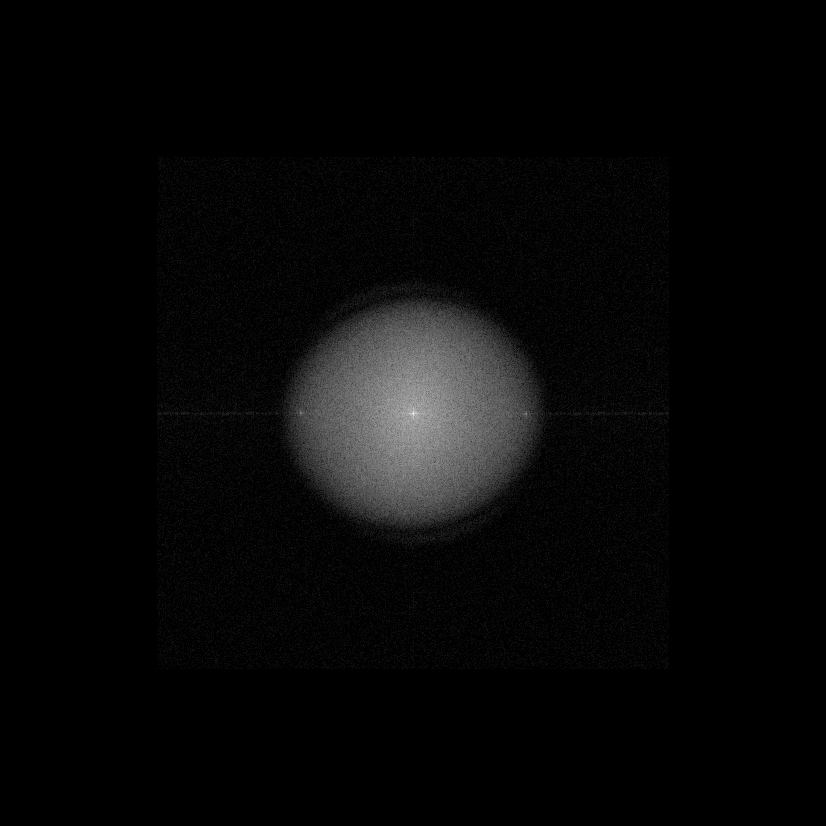
\includegraphics[width=\textwidth]{raw-fourier-transform}
	\caption{}\label{fig:raw-fourier-transform}
\end{subfigure}
\hfill
\begin{subfigure}[b]{0.49\textwidth}
	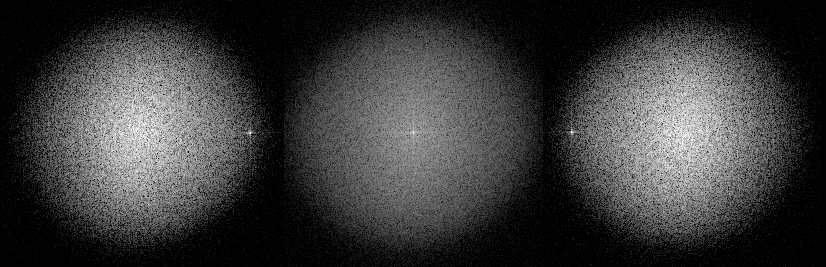
\includegraphics[width=\textwidth]{fourier-components}
	\caption{}\label{fig:fourier-components}
\end{subfigure}

\begin{subfigure}[b]{0.49\textwidth}
	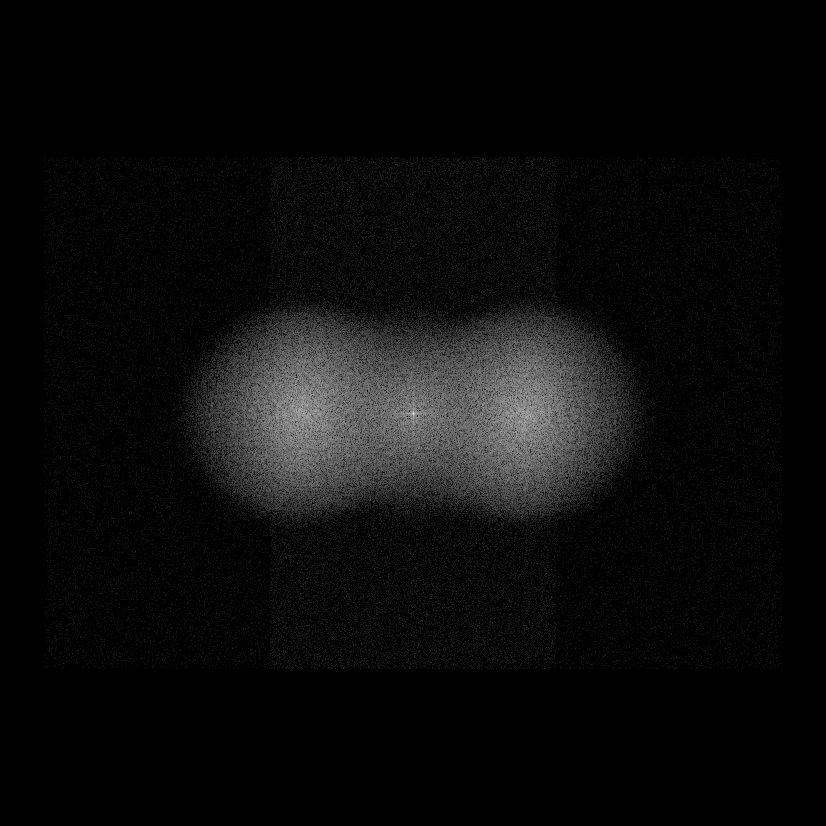
\includegraphics[width=\textwidth]{x-resolution-doubling}
	\caption{}\label{fig:x-resolution-doubling}
\end{subfigure}
\hfill
\begin{subfigure}[b]{0.49\textwidth}
	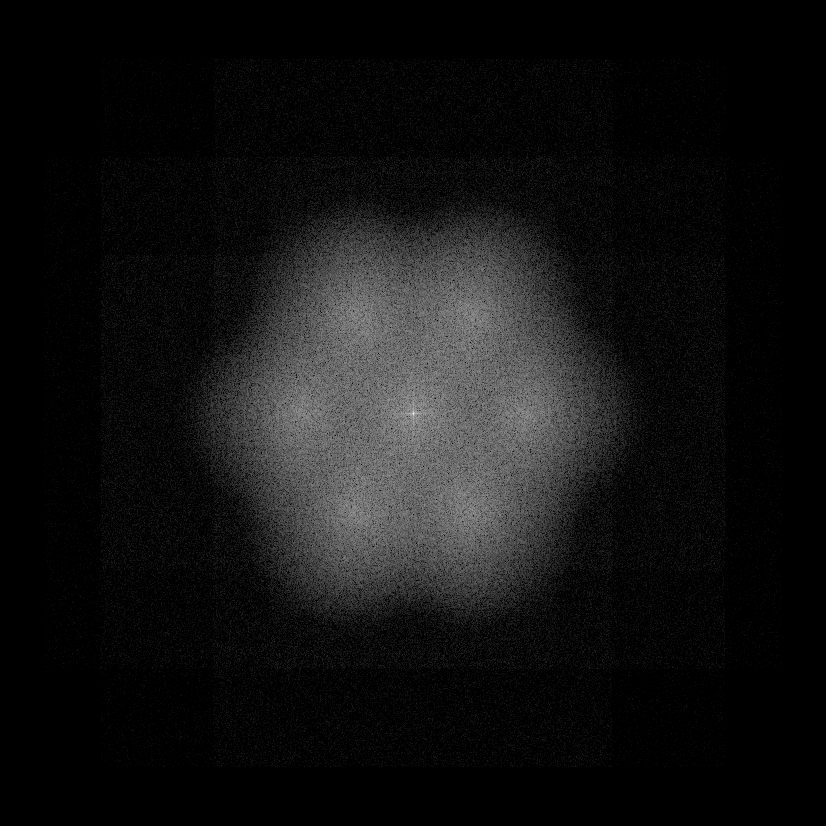
\includegraphics[width=\textwidth]{isotropic-SIM-fourier}
	\caption{}\label{fig:isotropic-SIM-fourier}
\end{subfigure}
\caption[LAG SIM: Reconstruction of SIM images takes place in Fourier space]{(a) shows the 2D Fourier transform of a raw SIM image, where the 3 delta peaks from the sine wave illumination pattern can be clearly seen as bright spots. (b) shows the separated components, after extraction by Equation~\ref{eq:matrix-inversion}. (c) shows the components shifted into the correct position in Fourier space, ready for inverse Fourier transforming - but this would only provide resolution enhancement in the x-direction. (d) shows the full Fourier space reconstruction generated from 3 rotations of the SIM pattern, requiring a total of 9 images. The full Fourier space reconstruction has an OTF which has local peaks and is not rotationally symmetric, necessitating the Wiener filtering scheme described in Equation~\ref{eq:wiener-filtering}.}
\label{fig:fourier-reconstruction}
\end{figure}

The same structured illumination microscopy (SIM) used for optical sectioning can be re-purposed for surpassing the diffraction limit. 
First discussed by Lucosz [1963], and then more explicitly described by Heintzmann [1998 in proceedings] for sinusoidal illumination patterns, the first experimental result showing 2D isotropic resolution doubling with 9 raw image acquisitions was published by Gustafsson in \num{2000}. 
Heintzmann shows that if we take the Fourier transform of the acquired images shown in Equation~\ref{eq:wilson-illumination}, we obtain the set of images shown in Equation~\ref{eq:heintzmann-fourier}, where \^{}-symbols represent 2D Fourier transforms of their equivalent variables, and $k_x$ is the Fourier variable of $x$, that is $f(x) \Leftrightarrow \hat{f}(k_x)$. 
Note that $W$ has been replaced with its underlying components $P\otimes S$, where $\hat{P}$, the Fourier transform of the PSF, is known as the optical transfer function (OTF). 

\begin{equation} \label{eq:heintzmann-fourier}
\hat{I_i} = \hat{P} \hat{S} \otimes \left( \delta \left( k_x \right) + \frac{m}{2} e^{j\phi_i} \delta \left( k_x + t \right) + \frac{m}{2} e^{-j\phi_i} \delta \left( k_x - t \right) \right) 
\end{equation}

Each acquired raw image contains contributions from each of 3 shifted Fourier components. 
Remembering $i=\left\lbrace1,2,3\right\rbrace$, these Fourier components can be separated into individual images by solving the set of simultaneous equations for $\hat{S}\otimes\delta \left( k_x \right)$, $\hat{S}\otimes\delta \left( k_x + t \right)$, and $\hat{S}\otimes\delta \left( k_x - t \right)$ with matrix inversion, as shown in Figure~\ref{fig:fourier-components} and Equation\ref{eq:matrix-inversion} [Wicker 1998?]. 
Assuming phase steps are all equal, performing a 3D Fourier transform of the phase-stepped raw images stacked in the 3rd dimension produces the same result. [Gustafsson 2000?]

\begin{equation} \label{eq:matrix-inversion}
\begin{bmatrix} \hat{S}\left(k_x\right) \\ \hat{S}\left(k_x+t\right) \\ \hat{S}\left(k_x+t\right) \end{bmatrix} = 
\begin{bmatrix}
1 & \frac{m}{2}\exp\left(-0j\right) & \frac{m}{2}\exp\left(0j\right) \\ 
1 & \frac{m}{2}\exp\left(-\frac{2j}{3}\right) & \frac{m}{2}\exp\left(\frac{2j}{3}\right) \\ 
1 & \frac{m}{2}\exp\left(-\frac{4j}{3}\right) & \frac{m}{2}\exp\left(\frac{4j}{3}\right)
\end{bmatrix}^{-1}
\begin{bmatrix} \hat{I_1} \\ \hat{I_2} \\ \hat{I_3} \end{bmatrix}
\end{equation}

To complete the reconstruction, the separated Fourier components must be placed at in the correct position in Fourier space, as determined by $t$. 
Assuming the sinusoidal illumination pattern is generated by the same lens used for imaging the sample, the highest frequency sine wave which can be generated will correspond to delta peaks at the edge of the microscope's support in Fourier space, shown in Figure~\ref{fig:raw-fourier-transform}. 
When the components are shifted into the appropriate location, the support and resolution of the microscope doubles in the $x$ direction, as shown in Figure~\ref{fig:x-resolution-doubling}. 

To achieve isotropic 2D resolution doubling, the sinusoidal illumination pattern must be rotated to cover more area in Fourier space. 
Typically a total of three rotations are used, at \SI{60}{\deg} and \SI{120}{\deg} to the original pattern orientation. 
Performing the reconstruction procedure on all 9 images produces a Fourier space, as shown in Figure~\ref{fig:isotropic-SIM-fourier}, gives the desired isotropic resolution doubling. 

The final step for this reconstruction procedure is to inverse Fourier transform the reconstructed Fourier space image, producing an image with double the equivalent widefield resolution. 


\subsection{Refining the reconstruction algorithm}
The 2D OTF of a lens is a rotationally symmetric function which gradually reduces to zero as spatial frequency increases. 
A line profile through the OTF of an ideal lens in Figure~\ref{fig:microscope-OTF} shows that the higher the spatial frequency, the less resolving power the microscope has.
In a practical set-up, noise further limits the resolution at high frequencies, such that signal-to-noise ratio decreases as spatial frequency increases. 

\begin{figure}[tbp]
\centering
\begin{subfigure}[b]{0.49\textwidth}
	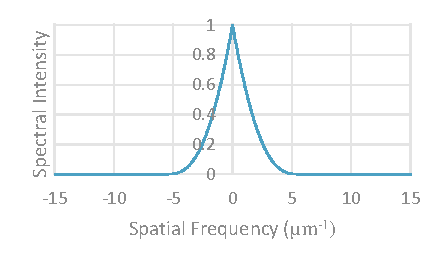
\includegraphics[width=\textwidth]{microscope-OTF}
	\caption{}\label{fig:microscope-OTF}
\end{subfigure}
\hfill
\begin{subfigure}[b]{0.49\textwidth}
	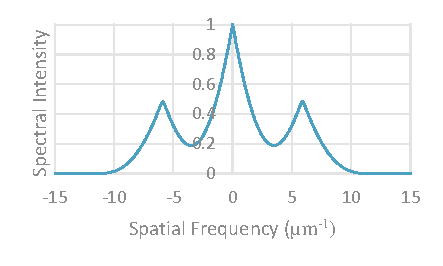
\includegraphics[width=\textwidth]{sim-OTF-peaks}
	\caption{}\label{fig:OTF-sim-peaks}
\end{subfigure}

~\newline
\begin{subfigure}[b]{0.49\textwidth}
	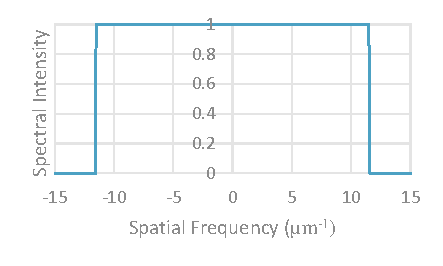
\includegraphics[width=\textwidth]{wiener-no-apo}
	\caption{}\label{fig:wiener-no-apo}
\end{subfigure}
\hfill
\begin{subfigure}[b]{0.49\textwidth}
	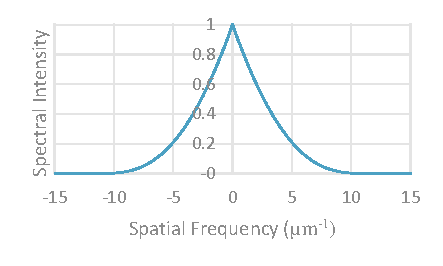
\includegraphics[width=\textwidth]{wiener-plus-apo}
	\caption{}\label{fig:wiener-plus-apo}
\end{subfigure}

~\newline
\begin{subfigure}[b]{0.49\textwidth}
	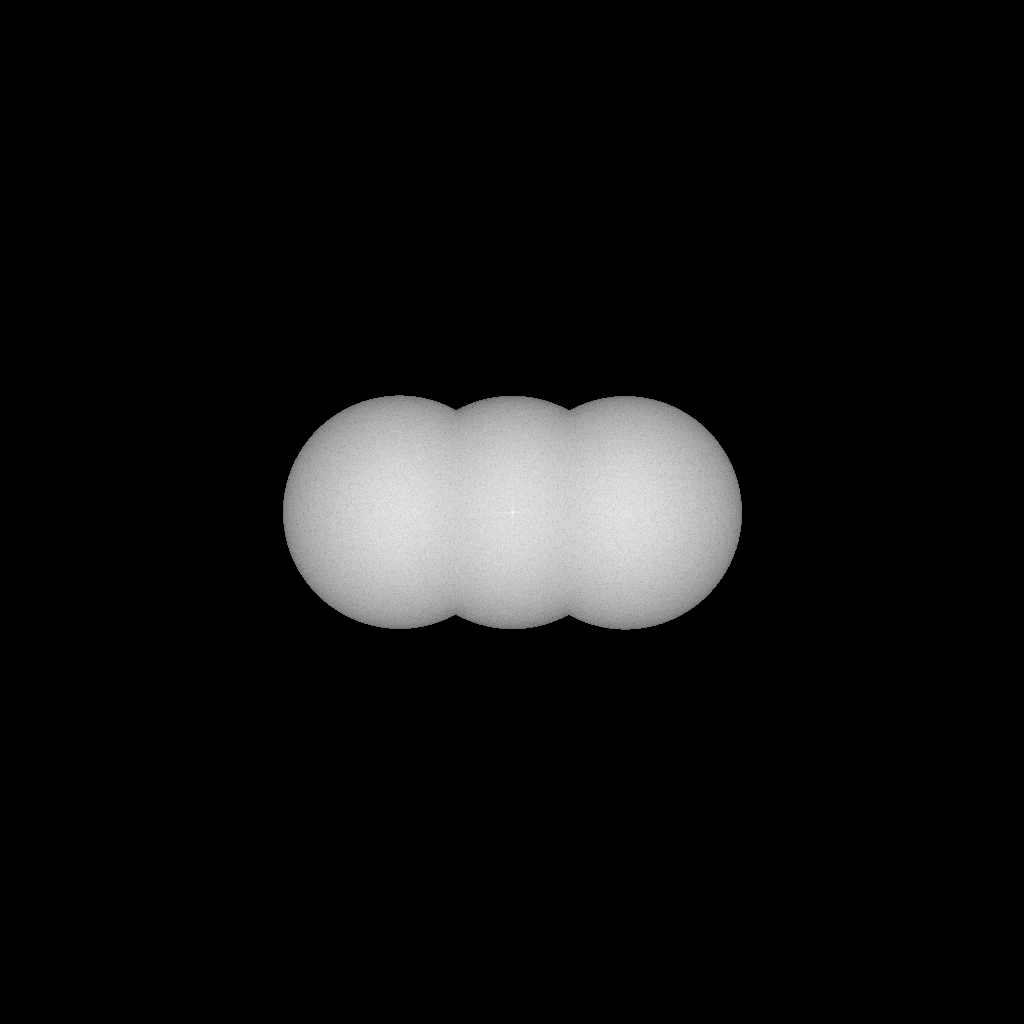
\includegraphics[width=\textwidth]{wienered-x-fourier}
	\caption{}\label{fig:wienered-x-fourier}
\end{subfigure}
\hfill
\begin{subfigure}[b]{0.49\textwidth}
	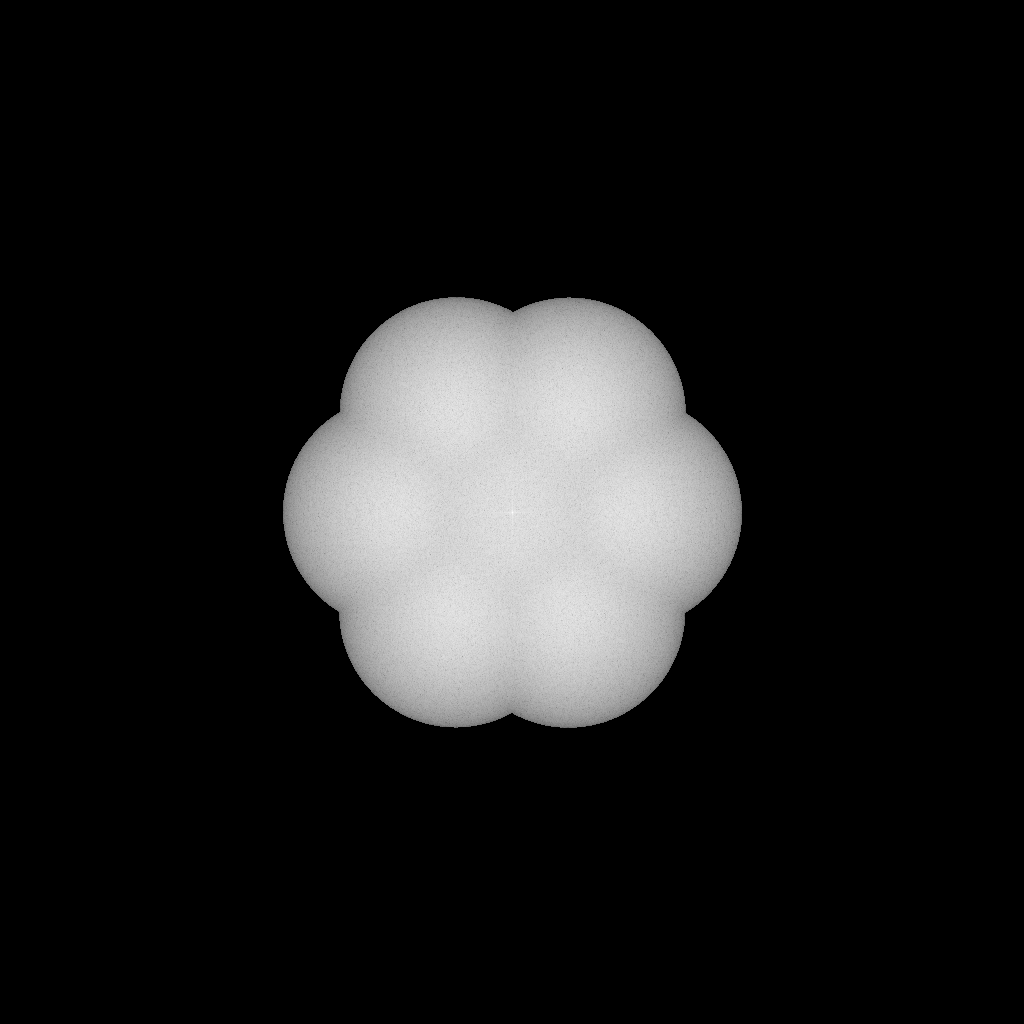
\includegraphics[width=\textwidth]{wienered-iso-fourier}
	\caption{}\label{fig:wienered-iso-fourier}
\end{subfigure}
\caption[LAG SIM: Wiener filtering of the SIM OTF is required for artefact-free reconstruction]{(a) shows the rotationally-averaged OTF of an ideal lens, which is equivalent to a cross-section through the 2D OTF due to rotational symmetry. After SIM reconstruction, (b) shows that local peaks appear in the OTF, due to shifting in Fourier space; furthermore, the OTF is no longer rotationally symmetric, producing characteristic SIM artefacts. The Wiener filtering scheme described in Equation~\ref{eq:wiener-filtering} produces a flat OTF shown in (c), with equal power at all frequencies; however the sharp cutoff produces ringing artefacts after Fourier transforming into real space. (d) shows the apodisation filter $A\left(\textbf{k}\right)$ which is applied to the OTF to reduce ringing artefacts, and closely resembles the widefield OTF shown in (a). (e) and (f) show the same shifted Fourier components as Figures~\ref{fig:x-resolution-doubling} and \ref{fig:isotropic-SIM-fourier}, but reconstructed through a Wiener filter to remove local peaks in the OTF.}
\label{fig:sim-OTFs}
\end{figure}

The signal-to-noise ratio has a particularly dramatic effect in SIM. 
Since each frequency component $\hat{S}_i$ is multiplied by the microscope OTF, the shifting shown in Figure~\ref{fig:fourier-components} results in an overall OTF which does not gradually decrease, but rather has peaks at certain frequencies, as shown in Figure~\ref{fig:OTF-sim-peaks}. 
These peaks translate directly to frequency peaks in the signal-to-noise ratio, therefore the noise pattern in the reconstructed image is no longer white noise with equal power at all frequencies. 
Furthermore, it can be seen in Figure~\ref{fig:isotropic-SIM-fourier} that the reconstructed SIM OTF is not rotationally symmetric. 
These two aspects combine to cause characteristic hexagonal noise artefacts in reconstructed SIM images. 

To reduce these artefacts, Fourier components are reconstructed through a de-noising algorithm.
The most common practice is to combine the frequency components through a generalised Wiener filter, as shown in Equation~\ref{eq:wiener-filtering} [Gustafsson 2008], to produce the reconstructed image $\hat{I_R}$. 
Note that this equation now describes the general 2D or 3D case, where $\mathbf{k}$ is a vector of Fourier variables and $\mathbf{p}$ is a vector in the direction of the sinusoidal illumination pattern for each direction $d$. 
$w^2$ is a constant, adjusted empirically depending on the level of noise in the image, and $A\left(\mathbf{k}\right)$ is an apodisation function. 

\begin{equation} \label{eq:wiener-filtering} 
\hat{I_R} = \frac{\sum_{d,i}\hat{P}^*\left(\mathbf{k} + \phi_i\mathbf{p}_d\right) \hat{S}_{d,i}\left(\mathbf{k} + \phi_i\mathbf{p}_d\right)} {\sum_{d,i}\abs{\hat{P}\left(\mathbf{k} + \phi_i\mathbf{p}_d\right)}^2 + w^2} A\left(\mathbf{k}\right)
\end{equation}

If $A\left(\mathbf{k}\right)=1$, this reconstruction scheme removes the decaying characteristic of the OTF, instead making a flat top-hat filter shown in Figure~\ref{fig:wiener-no-apo} which suddenly cuts off at the doubled resolution limit. 
This can also be seen in Figures~\ref{fig:wienered-x-fourier} and \ref{fig:wienered-iso-fourier}, where the Fourier space image now has equal spectral intensity across the reconstructed OTF. 
However, because the Fourier transform of a top-hat function is a sinc function, this causes ringing artefacts in the reconstructed image. 
The apodisation function $A\left(\mathbf{k}\right)$ is therefore chosen as a filter which decays from the 0 frequency to the new resolution limit, for example a Gaussian filter. [cite gross JLS ER paper]

More recent research [cite cite cite] suggests improvements to generalised Wiener filtering, and a detailed discussion of alternative filtering schemes follows in Section~\ref{sec:recon} of this chapter. 


\subsection{Aims for LAG SIM}
When I arrived in the Laser Analytics Group (LAG) a SIM microscope designed by Laurie Young was reaching the end of its practical life.
Issues with device degradation, detailed in Section~\ref{sec:lagsim-pockels}, limited the imaging speed to \SI{0.1}{\hertz}.
Furthermore, a complicated ensemble of software required an expert user to operate the microscope.

A physical relocation of the laboratory in 2016 provided the ideal opportunity to rebuild the microscope and the associated control software. The first priority was to restore the microscope to \SI{11}{\hertz} imaging speed. Once this was achieved, a list of several other aims were devised: 
\begin{enumerate}
	\item Provide an easy method to switch between optical sectioning SIM and resolution-doubling SIM in TIRF (Sections~\ref{sec:hardware} and \ref{sec:labview}). 
	\item Split the fluorescence emission light at the output of the microscope to facilitate simultaneous capture of multiple colour channels (Section~\ref{sec:lagsim-path}). 
	\item Re-write the control software to make the microscope user-friendly enoguh for a non-expert user to operate unsupervised (Section~\ref{sec:labview}).
	\item Design reconstruction software to allow users to quickly reconstruct artefact-free images without detailed knowledge of reconstruction algorithms (Section~\ref{sec:recon}). 
\end{enumerate}

As well as detailing solutions to these challenges, this chapter also presents a showcase of various biological experiments performed with LAG SIM. 
Section~\ref{sec:sim-showcase} can therefore be used a collection of case study examples for anyone wishing to run similar studies. 

\section{SIM hardware} \label{sec:hardware}
\subsection{Optical path design} \label{sec:lagsim-path}
As part of his PhD work from 2012-2016, Dr. Laurie Young designed and built a SIM microscope in the Laser Analytics Group~\cite{young2016guide}. 
The current SIM setup in the Laser Analytics Group (`LAG SIM') is based heavily on this original design, but with several modifications which were implemented by me when the Group moved location in February 2017. 

\begin{figure}[p]
\centering
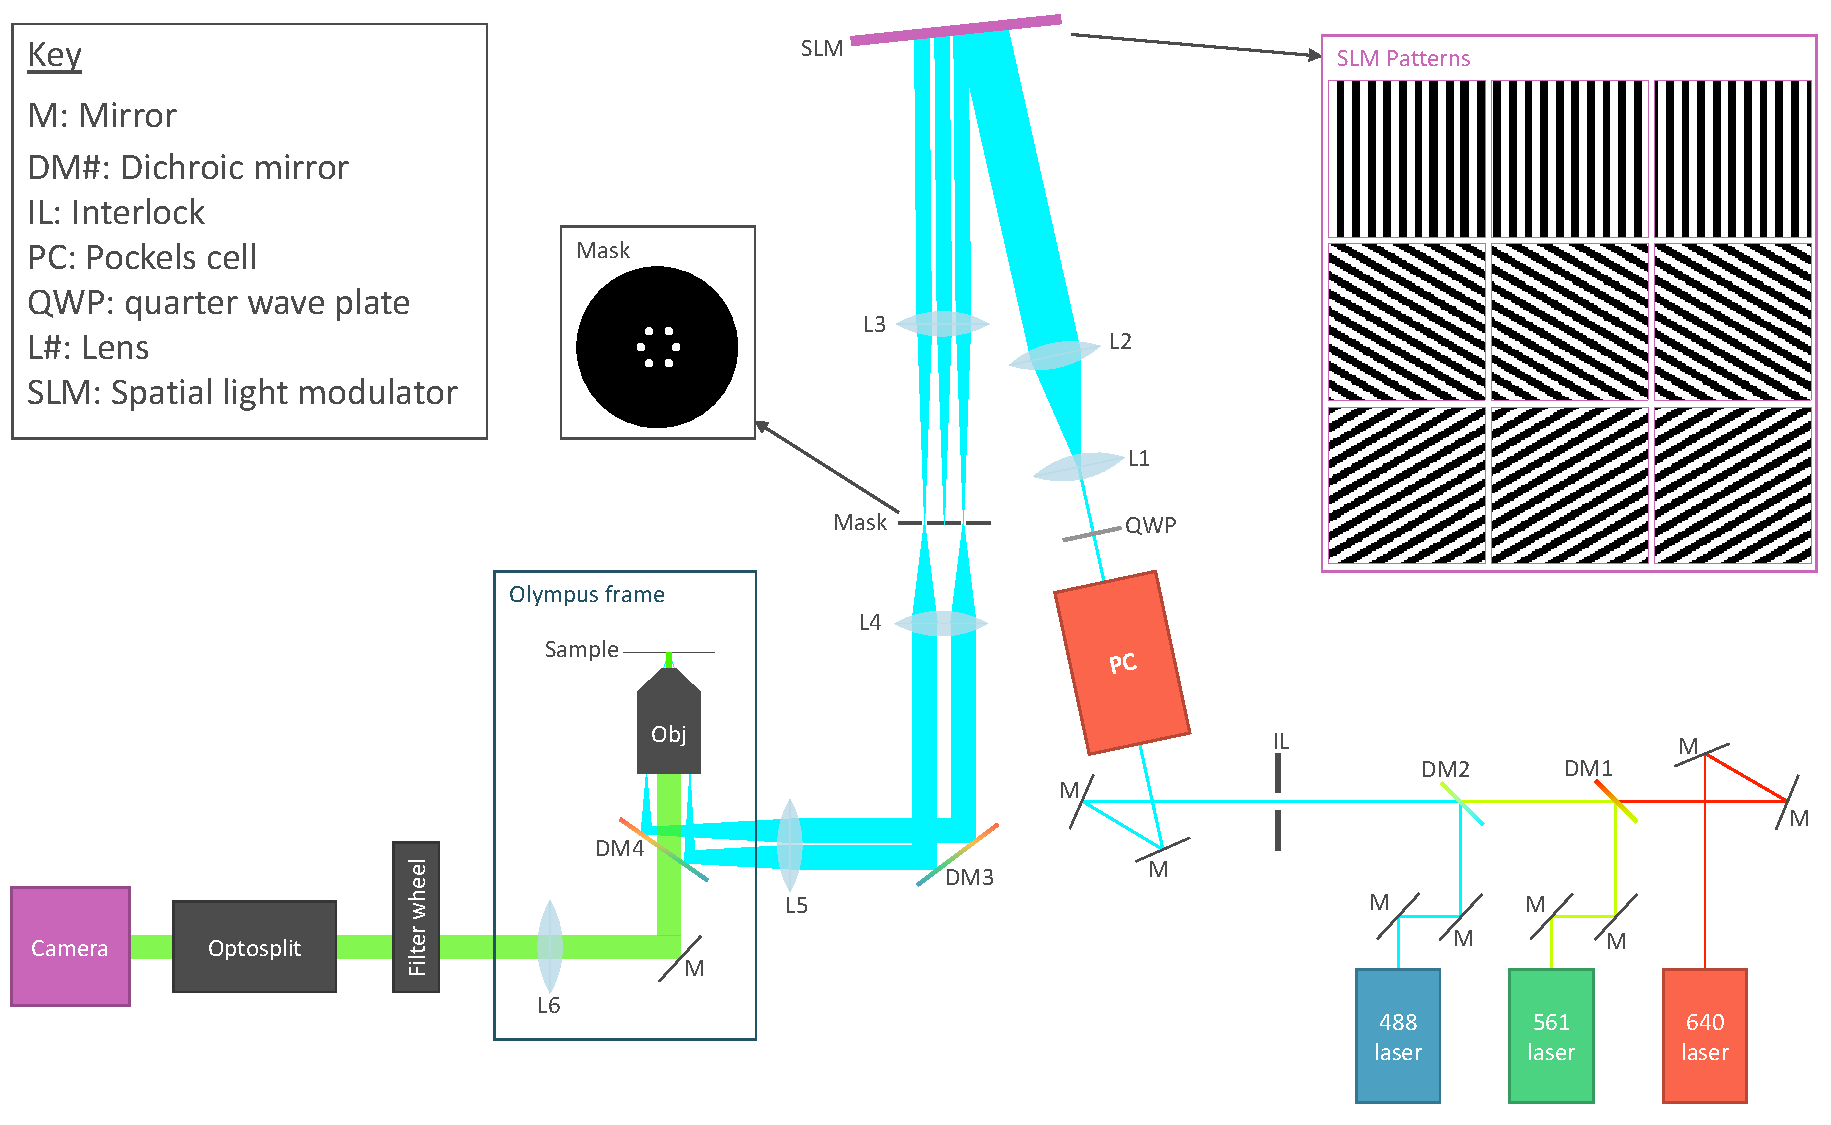
\includegraphics[angle=90, width=0.75\textwidth]{sim-optical-path}
\caption[LAG SIM: Optics pattern laser light with a SIM pattern and apply polarisation rotation for optical sectioning and resolution enhancement]{The optical layout of the SIM aligns light from one of 3 lasers onto an optical path. The light passes through a Pockels cell and quarter wave plate for polarisation rotation, before a square-wave pattern is applied by a spatial light modulator. The patterned light is passed through a spatial mask in the Fourier plane to produce a sinusoidal pattern, which is relayed onto the sample. The objective lens collects fluorescent emission light,  which is filtered to remove any reflected excitation light before reaching the sCMOS camera.}
\label{fig:SIMpath}
\end{figure}

The optical path diagram is shown in Figure~\ref{fig:SIMpath}, and works as follows: laser light is generated by one of three lasers at a wavelength of \SI{488}{\nano\metre}, \SI{561}{\nano\metre}, or \SI{640}{\nano\metre}; its polarisation is aligned with the direction of the structured illumination pattern by a Pockels Cell and achromatic quarter-wave plate; it passes through a beam expander so that it fully covers the SLM display; it reflects and diffracts off the SLM display, which is displaying a binary diffraction grating; it passes through a `beam minimiser' (a beam expander in reverse) so that it is an appropriate size for the microscope lenses; it passes through a spatial filter at a Fourier plane, which removes all but the ±1 diffraction orders from the SLM diffraction; it reflects off of a dichroic mirror; it passes into the microscope's tube lens; it reflects off of a second dichoric mirror, which is perfectly matched to the first; and finally it passes into the objective lens and is focussed onto the sample. 

This effectively images a low-pass-filtered version of the SLM's diffraction grating onto the sample. 
The spatial filter means that the binary grating becomes a sinusoidal pattern, with the distance between peaks set by the period of the diffraction grating shown on the SLM display and the demagnification of the system from SLM to sample. 
An equivalent way of conceptualising this is to picture the two filtered beams of light entering the back aperture of the objective lens, such that they produce an interference pattern when they meet at the sample plane. 
The result is a sinusoidal illumination pattern at the sample plane, the orientation and period of which can be set by a binary pattern shown on the SLM. 

This SIM is a fluorescence microscope, so that (to a reasonable approximation) the amount of light emitted from a point in the sample is proportional to the amount of light illuminating that point, but the emission light is at a different wavelength to the illumination light. 
In the LAG SIM microscope, fluorescent emission light travels back through the objective lens, through the dichroic mirror and towards the camera to record a 2D image. 
Before it reaches the camera, it is filtered in one of two ways, to remove any reflected illumination light.
The first option is to use a filter wheel, which contains three filters appropriate for removing the illumination light and can be switched via a serial command from the computer. 
The second option is to use the Optosplit III from Cairn Research, which uses filter cubes to split the emission light into three paths which are imaged onto separate areas of the camera, facilitating simultaneous imaging of three colour channels.

The Optosplit facilitates a significant increase in speed for multicolour imaging. 
In this setup, the fastest speed at which the camera can reliably image without dropping frames is \SI{10}{\milli\second}. 
A SIM reconstruction requires 9 images, giving a total exposure time of \SI{90}{\milli\second} per channel; however switching channels with the filter wheel adds an additional \SI{100}{\milli\second} as the wheel rotates in the next filter and settles. 
For a 3-colour image using the filter wheel, the fastest SIM imaging rate is therefore \SI{570}{\milli\second} per frame, or \SI{1.75}{\hertz}. 
Using the Optosplit is over 6 times faster, giving the full \SI{11.1}{\hertz} imaging rate even for multicolour images.

Finally, an autofocus system between the microscope frame and filter wheel works with the z-control of the microscope stage to maintain a constant focus on the sample. 
This is useful in two scenarios. 
Firstly, when a timelapse sequence is captured over a number of hours, the microscope lens drifts downwards away from the sample. 
Without the autofocus system, this would result in a loss of focus; however by automatically moving the stage as the lens drifts, focus can be maintained over a period of days.
Secondly, if a large field of view is imaged, focus can be lost due to the cover glass not being perfectly flat. 
Again, the autofocus system holds focus over this full field of view, allowing large areas to be imaged. 


\subsection{Pockels Cell} \label{sec:lagsim-pockels}
In the SIM excitation path, a Pockels Cell is used to rotate the polarisation of the illumination light so that it is aligned with the sinusoidal SIM pattern. 

In SIM, it is important that the modulation contrast is as large as possible, that is, that the troughs of the sinusoidal illumination pattern are as dark as possible.
When the 9 raw images are computationally recombined, the signal-to-noise ratio of high-spatial-frequency components is directly proportional to the modulation contrast~\cite{oholleran2012polarization}.

Modulation contrast of fluorescence emission light can be degraded by a number of sources, including out-of-focus light and aberrations in the imaging system, which is unavoidable in thick samples. 
Furthermore, if we do not take care with the polarisation of the illumination light,  modulation contrast is degraded due to the effects of a high numerical aperture lens. 

For two waves to interfere, they must have the same polarisation. [says this on Wikipedia "Wave interference", need better reference.]
As light passes through a high numerical aperture lens, the polarisation state which is parallel to the meridional plane (p-polarised) is rotated; whereas the polarisation state perpendicular (s-polarised) is unaffected. 
To ensure that light from the two back-aperture spots arrive at sample plane with the same polarisation, it is therefore necessary that the light is entirely s-polarised. 

If the meridional plane is defined at an angle of \SI{0}{\degree} around the $\phi$ axis, aligned with the back-aperture spots when the SLM is showing a vertical SIM grating pattern, the incident light should be linearly polarised at $\phi=90\si{\degree}$ so ensure s-polarised light. 
However, for 2D isotropic resolution enhancement, the SIM pattern must also be rotated to $\pm60\si{\degree}$. 
For these patterns, the spots are no longer aligned with the meridional plane defined for $\phi=0\si{\degree}$, thus the $\phi=90\si{\degree}$ polarisation does not represent s-polarised light for these patterns. 
In order to maintain s-polarised light, thereby ensuring maximum pattern contrast, the polarisation must be rotated for each orientation of the SIM pattern. 

[Need an image in here showing a lens, the meridional plane, two spots from the SIM pattern, and how they rotate for a different SLM pattern)

The original SIM system, detailed in reference~\cite{young2016guide}, used a liquid crystal variable retarder (LCVR) from Meadowlark Optics [cite old magazine] to rotate the polarisation to align with the SLM's grating orientation. 
This suffered an unexpected problem where the laser beam damaged the liquid crystal material leaving a visible spot on the LCVR and no longer retarded the light, so the system no longer rotated polarisation. 
The product line has since been discontinued.
As an interim solution, an achromatic half-wave plate was mounted in a serial-controlled rotation stage in place of the LCVR. 
This setup successfully rotated the polarisation and ensured good modulation contrast, but was only able to image at \SI{0.1}{\hertz}. 

In order to restore the LAG SIM to \SI{11}{\hertz} imaging speed, we purchased a Pockels Cell from Conoptics. 
Similarly to the LCVR, this allows the retardation of one polarisation axis which, in combination with a quarter-wave plate, allows for rotation of linear polarisation.
The level of retardation is controlled by a voltage across the Pockels Cell, restoring polarisation rotation to the LAG SIM with no mechanical movement. 

\subsection{Pockels Cell Alignment}
To use the Pockels Cell as a polarisation rotator, light entering the cell must be linearly polarised and aligned at \SI{45}{\degree} to the fast axis of the device. 
The Pockels Cell from [?SOMEONE] was delivered with a Glan Taylor polariser appropriately aligned in the factory. 

To align the Pockels Cell to the rest of the system, the following procedure was devised: % Shown in figure?
\begin{enumerate}
	\item Place the Pockels Cell in 5-axis mount
	\item Coarsely align so that the beam passes through the centre of the Pockels Cell
	\item Using a power meter after the Pockels Cell, rotate the cell until power is maximised
	\item Adjust the tip-tilt of the Pockels Cell, maximising power again
	\item Insert the quarter-wave plate (QWP) into the beam path mounted in a rotation mount 
	\item With the power meter after the QWP, rotate the QWP until power is maximised
\end{enumerate}

Although this alignment procedure could be completed with any laser, for LAG SIM it is best to use the 561 laser, as this is the closest to the centre wavelength of the achromatic quarter-wave plate. 

The polarisation state of the light was measured to ensure the Pockels Cell was behaving as expected by using a linear polariser in a rotation mount as an analyser before the power meter. 
The laser emission entering the Pockels Cell was linearly polarised, with an extinction ratio of 1:[???] for the 561 laser. 
The Glan Taylor polariser theoretically increases the extinction ratio to >1:\num{100000}~\cite{bennett1995handbook}, although because it is attached to the Pockels Cell in the factory, this extinction ratio cannot be measured. 
Light exiting the Pockels Cell is circularly polarised; using the analyser found an extinction ratio of [1:1??]. 
Finally, the QWP restores the light to linear polarisation, but rotated compared to the input as determined by the voltage over the Pockels Cell. Extinction ratio at the output of the QWP was 1:[???]. 

\subsection{Pockels Cell Voltages}
The voltage across the Pockels Cell determines the amount of optical anisotropy in the cell, which in this setup is directly proportional to the polarisation rotation. 
The voltages required to control anisotropy are of the order of \SI{200}{\volt}. 
To achieve these voltages, an amplifier supplied by [THE COMPANY] takes a \SIrange{0}{2}{\volt} [check this] input and provides \SI{200}{\volt\/\volt} gain. 
The amplifier input voltage is generated by a National Instruments Digital to Analog Converter (DAC), which is controlled by a LabVIEW program. 

\begin{figure}[htbp!]
\centering
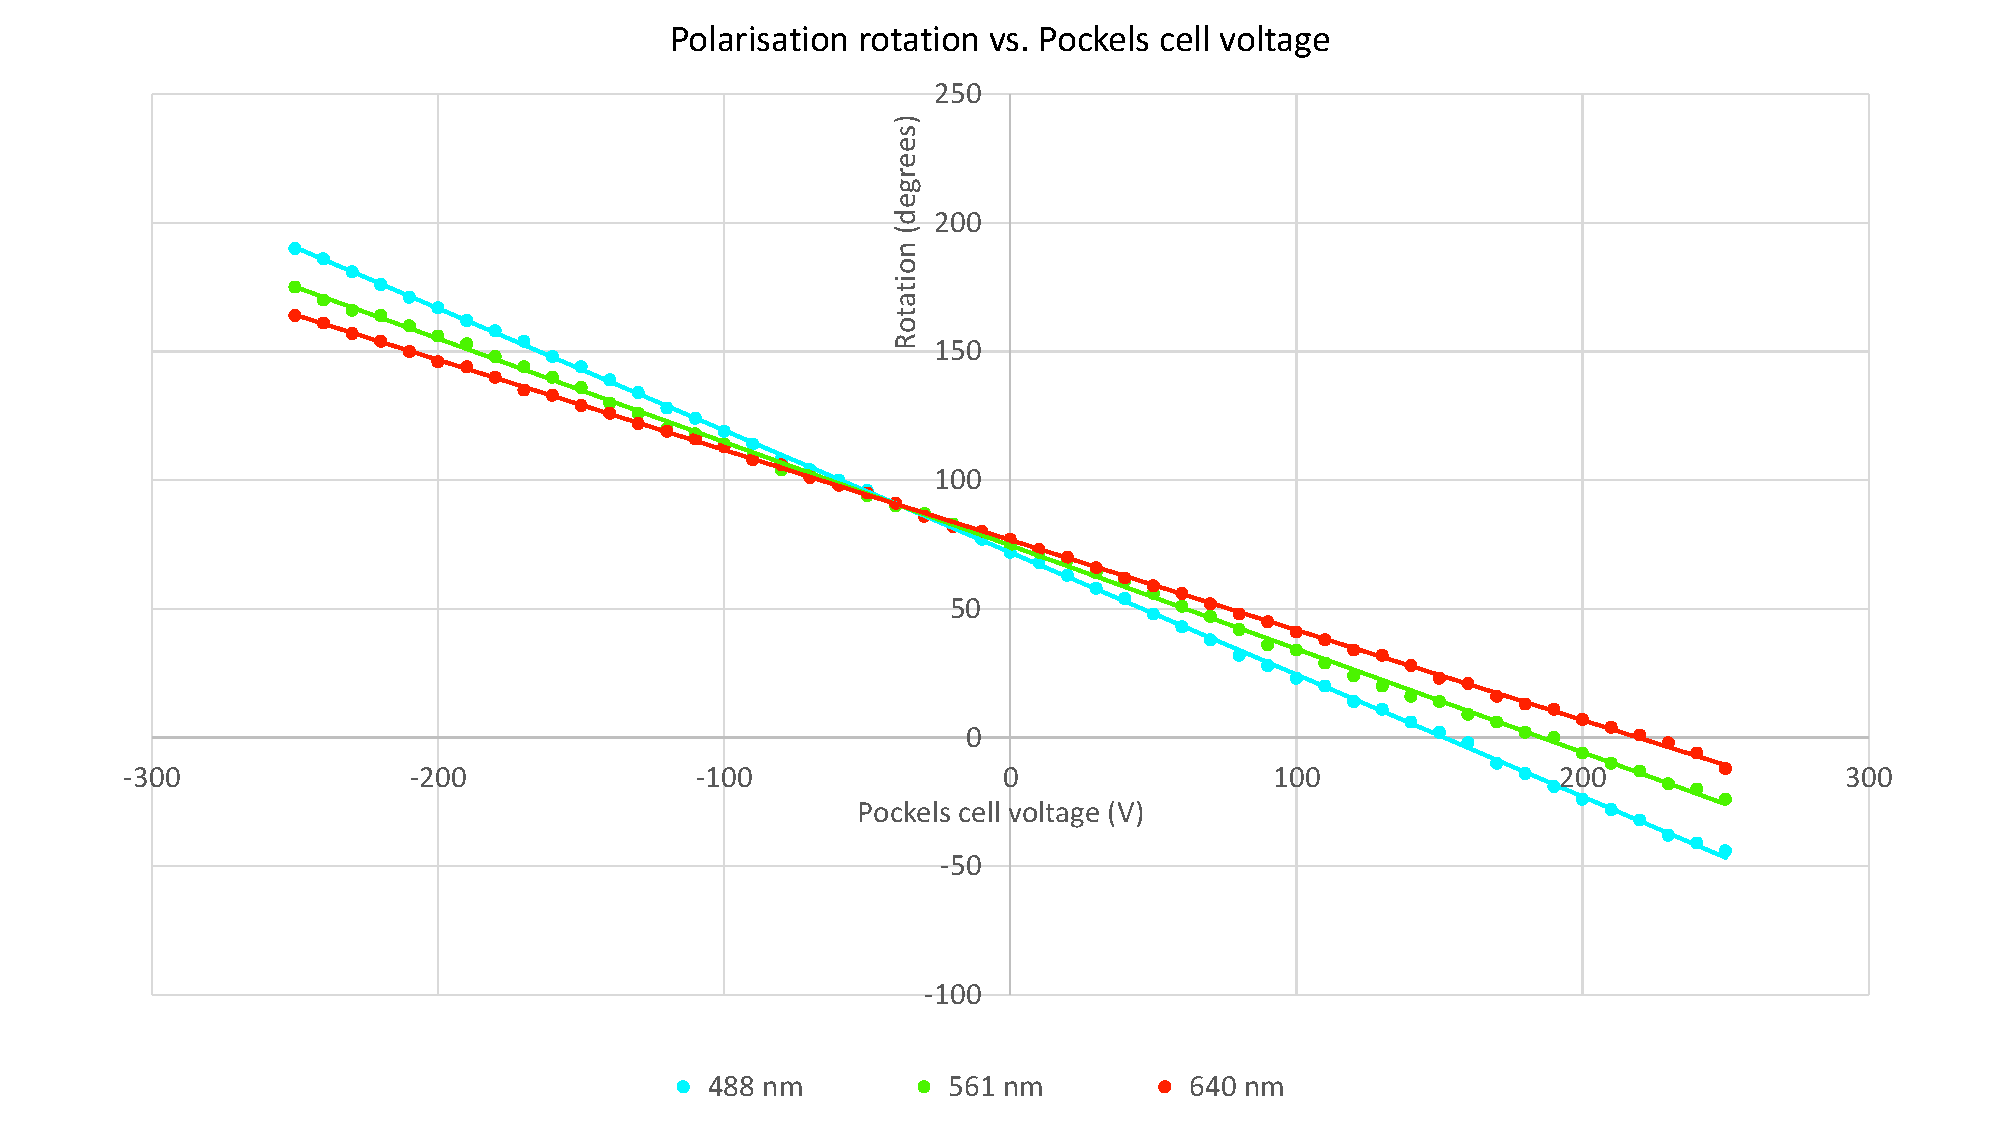
\includegraphics[width=1.0\textwidth]{pockels-voltage-vs-rotation}
\caption[LAG SIM: A Pockels cell is used to rotate the polarisation of laser light for maximum SIM pattern contrast]{When used in combination with a quarter wave plate, the voltage across the Pockels cell is proportional to polarisation rotation for each wavelength of laser light. Though the relationship is slightly different for each wavelength, at low voltages the gradients are similar enough that the~\SI{561}{\nano\metre} voltages can be used when the Optosplit is being used to image multiple channels simultaneously.}
\label{fig:pockels-voltage-rotation}
\end{figure}

Figure~\ref{fig:pockels-voltage-rotation} shows the relationship between voltage and polarisation rotation for the three laser lines used on the LAG SIM. 
Two useful properties of the Pockels cell are evident. 
Firstly, the device is able to provide a full \SI{360}{\degree} polarisation rotation, more than adequate for the $\pm60\deg$ required to align polarisation with the SIM pattern orientations. 
Secondly, to achieve a given rotation a similar voltage is required for all wavelengths. 
This is an especially important property for using the Optosplit, when all lasers are imaging the sample simultaneously. 

To calculate the voltages required to achieve maximum pattern contrast at each wavelength and orientation, a program was written in LabVIEW to sweep the Pockels' Cell voltage across the input range in steps of \SI{0.2}{\volt}. 
At each voltage step, 9 SIM images of sub-diffraction beads were recorded, and their contrast was measured by a MATLAB script. 
The contrast was plotted against voltage, as shown in Figure~\ref{fig:pockels-contrast}.
This procedure was repeated for every pattern orientation and every wavelength, producing a table of optimal voltages for each combination, which can be seen in Figure~\ref{fig:lagsimLabview}. 

\begin{figure}[htbp!]
\centering
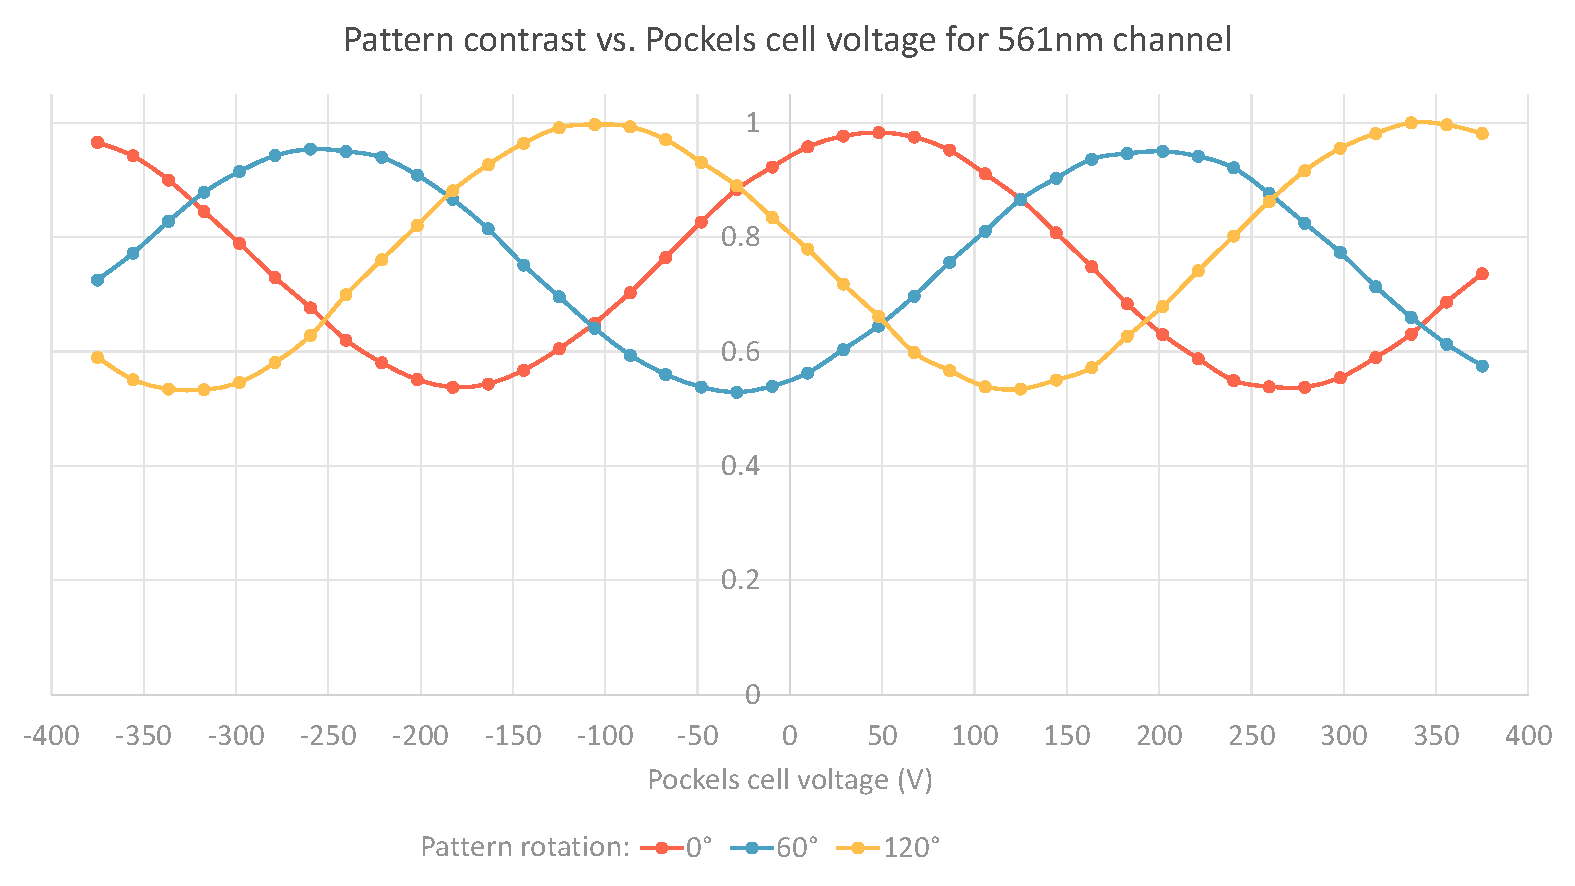
\includegraphics[width=1.0\textwidth]{pockels-contrast}
\caption[LAG SIM: Measurements of a bead sample reveal the ideal Pockels cell voltages for maximum pattern contrast]{Pattern contrast was measured on a \SI{100}{\nano\metre} bead sample as the voltage was swept from \SIrange{-375}{375}{\volt} to find the voltage which gave maximum contrast. The process was repeated for each rotation of the sinusoidal SIM pattern, and for each wavelength of light. }
\label{fig:pockels-contrast}
\end{figure}

% Some kind of concluding paragraph, pointing out that now we have the pockels cell we can do super duper fast imaging. 

% Can I spin this whole thing to say that by using a Pockels cell, we were able to use the optosplit for SIM? And quote Strohl et al about high frame rates reqired for SIM? 
% Probably ;) 




\section{LabVIEW Hardware Control} \label{sec:labview}
\subsection{Control requirements} \label{sec:SIMsteps}
The LAG SIM has a number of hardware components which must all work together to acquire a set of images appropriate for SIM reconstruction.
Specifically, the following sequence of events must take place:
\begin{enumerate}
	\item Set filter wheel to correct position for the excitation and emission wavelengths
	\item\label{step:pockels} Set voltage across Pockels Cell for correct polarisation rotation
	\item Set SLM pattern to the correct orientation and phase
	\item Turn on the laser
	\item Open the camera shutter for the exposure time
	\item Close the camera shutter
	\item Turn off the laser
	\item\label{step:record} Record the image
\end{enumerate}
Steps \ref{step:pockels} to \ref{step:record} must be repeated for each of the 9 illumination patterns, and the entire process then repeated for additional colour channels if the Optosplit is not being utilised. 
For a time series, this entire process must then be repeated for the required number of frames; for a z-stack, the height of the stage must also be adjusted before repeating the process. 

The original SIM, detailed in [cite JOVE, again!], used a separate software program for controlling each piece of hardware. 
This caused a number of problems: firstly, setting up experiments was an complicated process prone to human errors; and secondly, making modifications to the imaging parameters during an imaging session was difficult and time-consuming. 
When imaging live-cell biology, there is a real impetus to image quickly, as cells are becoming unhealthy and soon dying on the microscope stage. 

Furthermore, the complicated system meant that only one person in the LAG had the knowledge to gather images from the SIM. 
This meant that any biological experiments which would benefit from SIM required my direct supervision, so that many projects were not able to use the SIM, and I personally had little time for other research aims.
There was a clear need for a new, unified SIM interface, which could be used by non-expert users with minimal training. 

\subsection{LAG SIM Interface}
The new interface was built in LabVIEW. 
Although each hardware component came with its own control software, all components could also be controlled either through serial commands, analog voltages, or transistor-transistor logic (TTL) levels. 
As a graphical language with hardware control in mind, LabVIEW provides easy-to-use built-in blocks to fulfil each of these functions, as well as a clear visual representation of a sequence of control events.
Furthermore it makes designing user interfaces a straightforward process, allowing a programmer to create a user-friendly program for the end user. 
This made LabVIEW an ideal candidate for building an accessible program for controlling the LAG SIM.

The LAG SIM interface is shown in Figure~\ref{fig:lagsimLabview}.
The two key main areas of use are the Live Mode area and the Acquire tab, although for the sake of completeness each tab is detailed in this section. 

\begin{figure}[p]
\centering
\begin{subfigure}[b]{0.6\textwidth}
	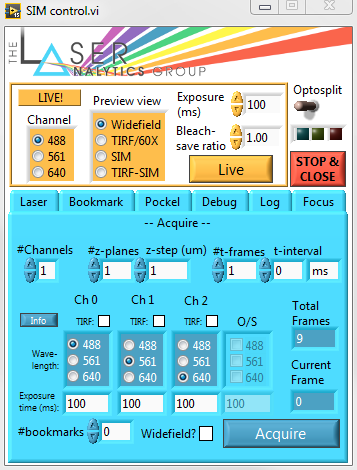
\includegraphics[width=\textwidth]{lagsimLabviewAcq}
	\caption{}\label{fig:fpbLabviewAcq}
\end{subfigure}

~\newline
\begin{subfigure}[b]{1.0\textwidth}
	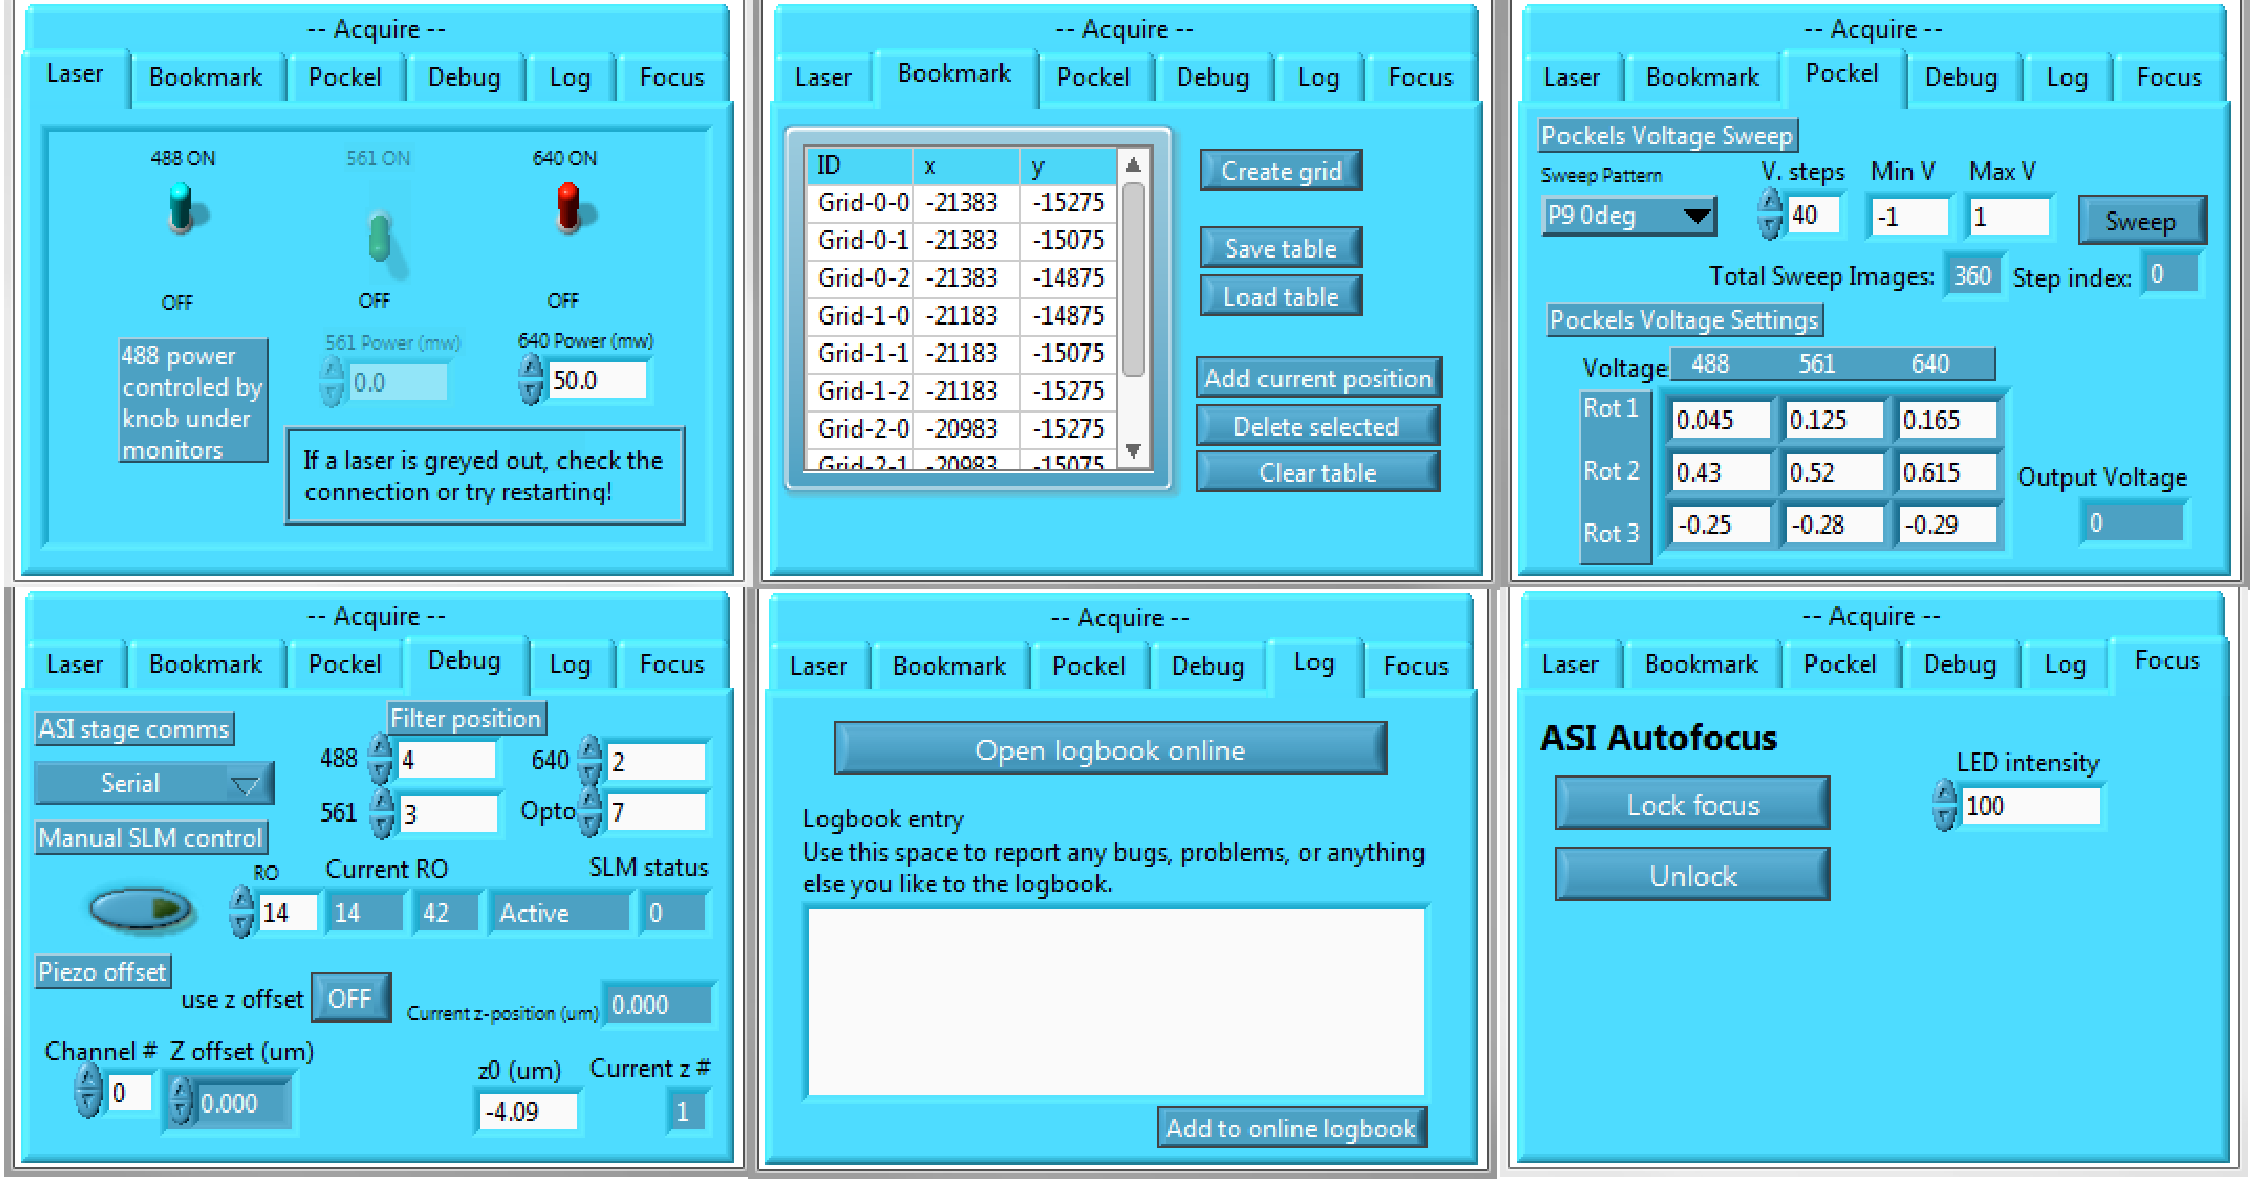
\includegraphics[width=\textwidth]{lagsimLabviewOthers}
	\caption{}\label{fig:fpbLabviewTabs}
\end{subfigure}
\caption[LAG SIM: The LabVIEW user interface for controlling LAG SIM is designed for operation by non-expert users]{The LabVIEW user interface used to control the LAG SIM has been designed for operation by a non-expert user, with advance tasks hidden in the extra tabs shown in (b). } % Needs a few more words actually 
\label{fig:lagsimLabview}
\end{figure}

\subsection{Live tab} \label{sec:lagsimLive}
The live tab is always visible whenever the LAG SIM Control software is open. 
It works in conjunction with the HCImage camera software provided by Hamamatsu, which provides a live display of the camera chip. 
% A few more details about the camera software at this point? Maybe I can save that for Acquire mode

In live mode, the illumination wavelength can be changed with the radio buttons or with the F2, F3 and F4 keys for fast, mouse-free operation. 
This allows users to quickly identify cells in one channel, for example with a fluorescent nucleus marker, and confirm presence of another marker in the second channel.
This fast channel switching minimises photobleaching when panning for healthy cells to image in detail. 
% This is surprisingly useful, see supplementary video? 

Another live-mode feature designed to reduce bleaching is the so-called `bleach-save ratio.' 
This is a number between 0 and 1 which switches off the laser for a fraction of the exposure time. 
By setting the exposure time and bleach-save ratio as small as possible while still being able to find healthy cells, the level of light the sample is exposed to can be minimised.
This is especially important in live-cell biology, where excess light can cause phototoxic effects bringing about cell death. 

The illumination pattern used for live mode will usually be a pseudo-widefield mode, which emulates widefield illumination by dithering all three phases of a particular orientation over one exposure time of the camera. 
True epi-illumination is not possible on the LAG SIM due to the spatial mask in the Fourier plane. 
The user can also choose to preview the SIM pattern by selecting the appropriate radio button; if the stripe pattern is visible, this is a good indication that later reconstruction into a resolution-enhanced image will be successful. 
If the \SI{1.49}{\numaperture} TIRF lens is used, then selecting the TIRF radio button sets the SLM pattern such that the ±1 diffraction spots hit the TIRF ring on the objective back aperture, leading to TIRF illumination at the sample. 
This can be done with the SIM pattern visible or in a dithered mode, as with non-TIRF illumination. 

The Optosplit rocker sets the software up for imaging with the Optosplit. [cite] 
The Optosplit is a device on the output port of the microscope which contains two filter cubes and a set of mirrors so that each channel can be imaged simultaneously onto a separate 512$\times$512 area of the 2048$\times$2048 camera chip.
When the filter cubes are removed, and the Optosplit rocker is in the \texttt{OFF} position, the Optosplit has no effect and channels are imaged sequentially, with an appropriate filter for each channel loaded into position by the filter wheel. 
With Optosplit mode \texttt{ON}, however, the live-mode channel selection radio buttons become checkboxes, so that each colour channel can be switched on and off independently. 
The Optosplit provides much faster imaging speeds, at the potential cost of cross-talk between colour channels. 
An example of Optosplit use is presented in Chapter~\ref{chap:ER}. % Should actually move most of this up, and just talk about the user interface here, maybe about assessing bleedthrough from shorter wavelengths to longer ones

This upper section of the user interface contains two more important components. 
A laser status indicator shows which lasers are currently exposing, an important safety feature so that users know it is safe to remove their sample after an imaging session. 
The \texttt{STOP \& CLOSE} button safely exits the control software, ensuring that the the lasers are switched off, the camera is finished exposing, and the voltage across the Pockels Cell is set to \SI{0}{\volt}. 
To ensure that this exit sequence runs when a user has finished their imaging session, the `\texttt{X}' close button in the window's title bar is disabled. 

\subsection{Acquire tab}
Once a healthy cell with the required staining has been located from live mode, it should be captured as a SIM image with the Acquire tab. 
With the default settings, this will capture a set of 9 raw SIM images following the steps described in Section~\ref{sec:SIMsteps}.
Additional settings in this tab allow a set of images to be captured for 3D z-stacks, timelapse imaging, and other multi-image acquisitions. 

If the number of z-steps is greater than 1, then the ASI stage will move in the axial direction at the end of every SIM acquisition by the value given in the z-step box. 
Since the axial resolution of the SIM is \SI{500}{\nano\meter} [check this!!], for a Nyquist-limited z-stack a z-step of \SI{200}{\nano\meter} should be used. 

To take a series of images over time, the t-frames should be set to greater than 1.
For observing fast, dynamic events, the t-delay should be set to \SI{0}{\milli\second}. 
Timelapse imaging, for example capturing an image every minute for an hour, can be achieved by setting the t-delay to \SI{60}{\second}, which will pause the software for the given amount of time at the end of each acquisition. 

Multi-channel imaging can be achieved either with or without the Optosplit. 
If the Optosplit switch is set \texttt{OFF}, and the number of channels is set to more than 1, the filter wheel will rotate the correct filter into position after each channel is captured. 
The exposure time of each raw SIM frame can be set per-channel, and the channel order can be changed with the radio buttons. 

Faster imaging can be achieved with the Optosplit. 
This sets the filter wheel to an empty filter, and filtering is performed with filter cubes in the Optosplit. 
In this mode, the choice of channels is controlled with checkboxes. 

The bookmarks number should be set to the number of bookmarks in the bookmarks table, or a lower number $N$ if the user only wants to capture the first $N$ bookmarked locations from the table. 
If bookmarks are not to be used, this value should be left at 0 - a value of 1 will move to the first bookmark listed in the bookmark table and capture an image there. 
Bookmarks are discussed in more detail in Section~\ref{sec:lagsimBookmarks}. 

The SIM microscope can be used to capture images in a pseudo-widefield mode, by dithering the SIM pattern as described in Section~\ref{sec:lagsimLive}. 
This is enabled by ticking the \texttt{Widefield} checkbox. 
This will enabled imaging with a widefield resolution at \SI{100}{\hertz}. 

Once the appropriate variables have been set for the acquisition, the total frames is displayed in the \texttt{Total frames} box. 
This number should be entered into the HCImage camera software, to prepare the camera for a high-speed image acquisition. 
Once the user has pressed \texttt{Start} in the HCImage software, the camera buffer is ready to receive images; then pressing \texttt{Acquire} in the LAG SIM software starts the acquisition process. 

A future version of the software could automate this final step, eliminating the need for the HCImage software.
This would require careful access to the camera data stream through LabVIEW. 


\subsection{Laser tab}
Laser control is integrated into the LAG SIM control software. 

At the launch of the software, the controls are greyed-out and disabled. 
When LabVIEW successfully connects to each laser, its controls become enabled, to switch the lasers on and off and change the power. 
Lasers are switched off automatically when the software is closed, for added safety when the microscope is unattended. 

Having fast and straightforward access to laser control is particularly useful for reducing light dosage in live mode.
Power can then be increased for acquisition to obtain the highest possible image quality. 

% Am I going to get 488 power sorted before I leave?! No. Just moved it to a nicer place. 

\subsection{Bookmark tab} \label{sec:lagsimBookmarks}
The LAG SIM LabVIEW program is able to store locations on the microscope slide as bookmarks.
If the number of bookmarks in the \texttt{Acquire} tab is set to greater than 0, the microscope stage will move before each acquisition to the next bookmarked position in the bookmark table. 
This is especially useful for imaging a collection of cells over a long period of time. 

The SIM user can pan around the microscope slide in \texttt{live mode} searching for healthy cells with good fluorescent labelling, and save them to the bookmark table by clicking \texttt{Add bookmark}. 
The location can be returned to by double-clicking on the table entry, or acquired sequentially and repeatedly in the \texttt{Acquire} tab. 

Furthermore this part of the software contains an option for creating bookmarks in a grid pattern. 
This can be utilised for imaging large areas, which are then stitched together to form one image, for example the whole mouse brain shown in Figure~\ref{fig:wholebrain}. 

\begin{figure}[p]
\centering
\includegraphics[angle=90, width=1.0\textwidth]{whole-brain}
\caption[LAG SIM: An image of a full mouse brain can be captured as a mosaic of images]{The bookmark mode offered by LAG SIM can be used to create tiled images, such as this 3-colour image of a mouse brain. Scalebar is \SI{500}{\micro\metre}}
\label{fig:wholebrain}
\end{figure}

\subsection{Focus} \label{sec:lagsimFocus}
Using the grid bookmark function to image large fields of view can fail if the coverglass or microscope stage is not perfectly flat, which is usually the case in all practical experiments. 
To keep the focus locked at the same distance from the sample, the `Lock focus' button begins the autofocus procedure. 
Assuming the autofocus sensor receives enough reflected signal from the infrared autofocus LED, the sample will be locked a fixed distance from the objective lens. 
If not, an error message is returned requesting the user to increase the LED power for a stronger signal. 
The system can also be used to maintain focus over a time period of hours to days, even as the objective lens drifts away from the sample. 

The autofocus is switched off with the `Unlock focus' button, releasing z-control back to the user. 

% Think I have a calibration tab, right? 
\subsection{Sweep} 
The Pockels cell retards one polarisation axis by an amount dependent on the voltage across it. 
In combination with a quarter wave plate, this allows for linear polarisation rotation necessary for the high pattern contrast required for SIM. 
The amount of retardation depends on the wavelength of light, therefore different wavelengths require different voltages to achieve the same polarisation rotation. 

To find the optimum voltage for each wavelength, functionality is built in to the \texttt{Sweep} tab to sweep the voltage from \SIrange{-1}{1}{\volt}, in a number of voltage steps. 
At each voltage, the SIM pattern's phase is swept and pattern contrast can be measured using a diffraction-limited bead sample. 
Pattern contrast is calculated with a MATLAB script to produce a graph as shown in Figure~\ref{fig:pockels-contrast}a, showing how pattern contrast changes with voltage. 

This gives a coarse estimation of the voltage required to achieve maximum pattern contrast. 
The sweep limits can then be adjusted either side of the coarse estimation to obtain an accurate voltage, shown in Figure~\ref{fig:pockels-contrast}b. 

This process must be repeated for each wavelength, and each rotation of the SIM pattern. 
Once the process is complete, the optimum voltages can be entered into the table, and will be applied to the Pockels cell during a SIM acquisition. 


\subsection{Debug}
A number of advanced user options are contained in the \texttt{Debug} tab. 
These extend the functionality of the microscope for non-conventional uses. 

The emission filters in the filter wheel change with excitation wavelength for use with commercially available fluorophores.
However, some samples - such as semiconducting perovskites - emit around \SI{750}{\nano\metre} when excited with \SI{488}{\nano\metre} light. 
Unconventional filters can be selected in this tab to image these samples. 

Manual SLM control gives the user direct control over the pattern displayed on the SLM. 
This means specialised patterns, such as a SIM pattern masked by a circle, or even 3 SIM patterns with different orientations overlayed, can be used.
These types of patterns are particularly useful for alignment of the system: overlaying 3 orientations of the SIM pattern produces 6 spots at the Fourier plane, which must be centred around the optical axis; therefore a coarse alignment can be performed using a translucent pinhole alignment tool on the microscope, as shown in Figure~\ref{fig:pinhole-alignment}. 
A fine alignment is then performed using the masked patterns, by ensuring the two circles overlap at the focal plane of the microscope. 

\begin{figure}[htbp!]
\centering
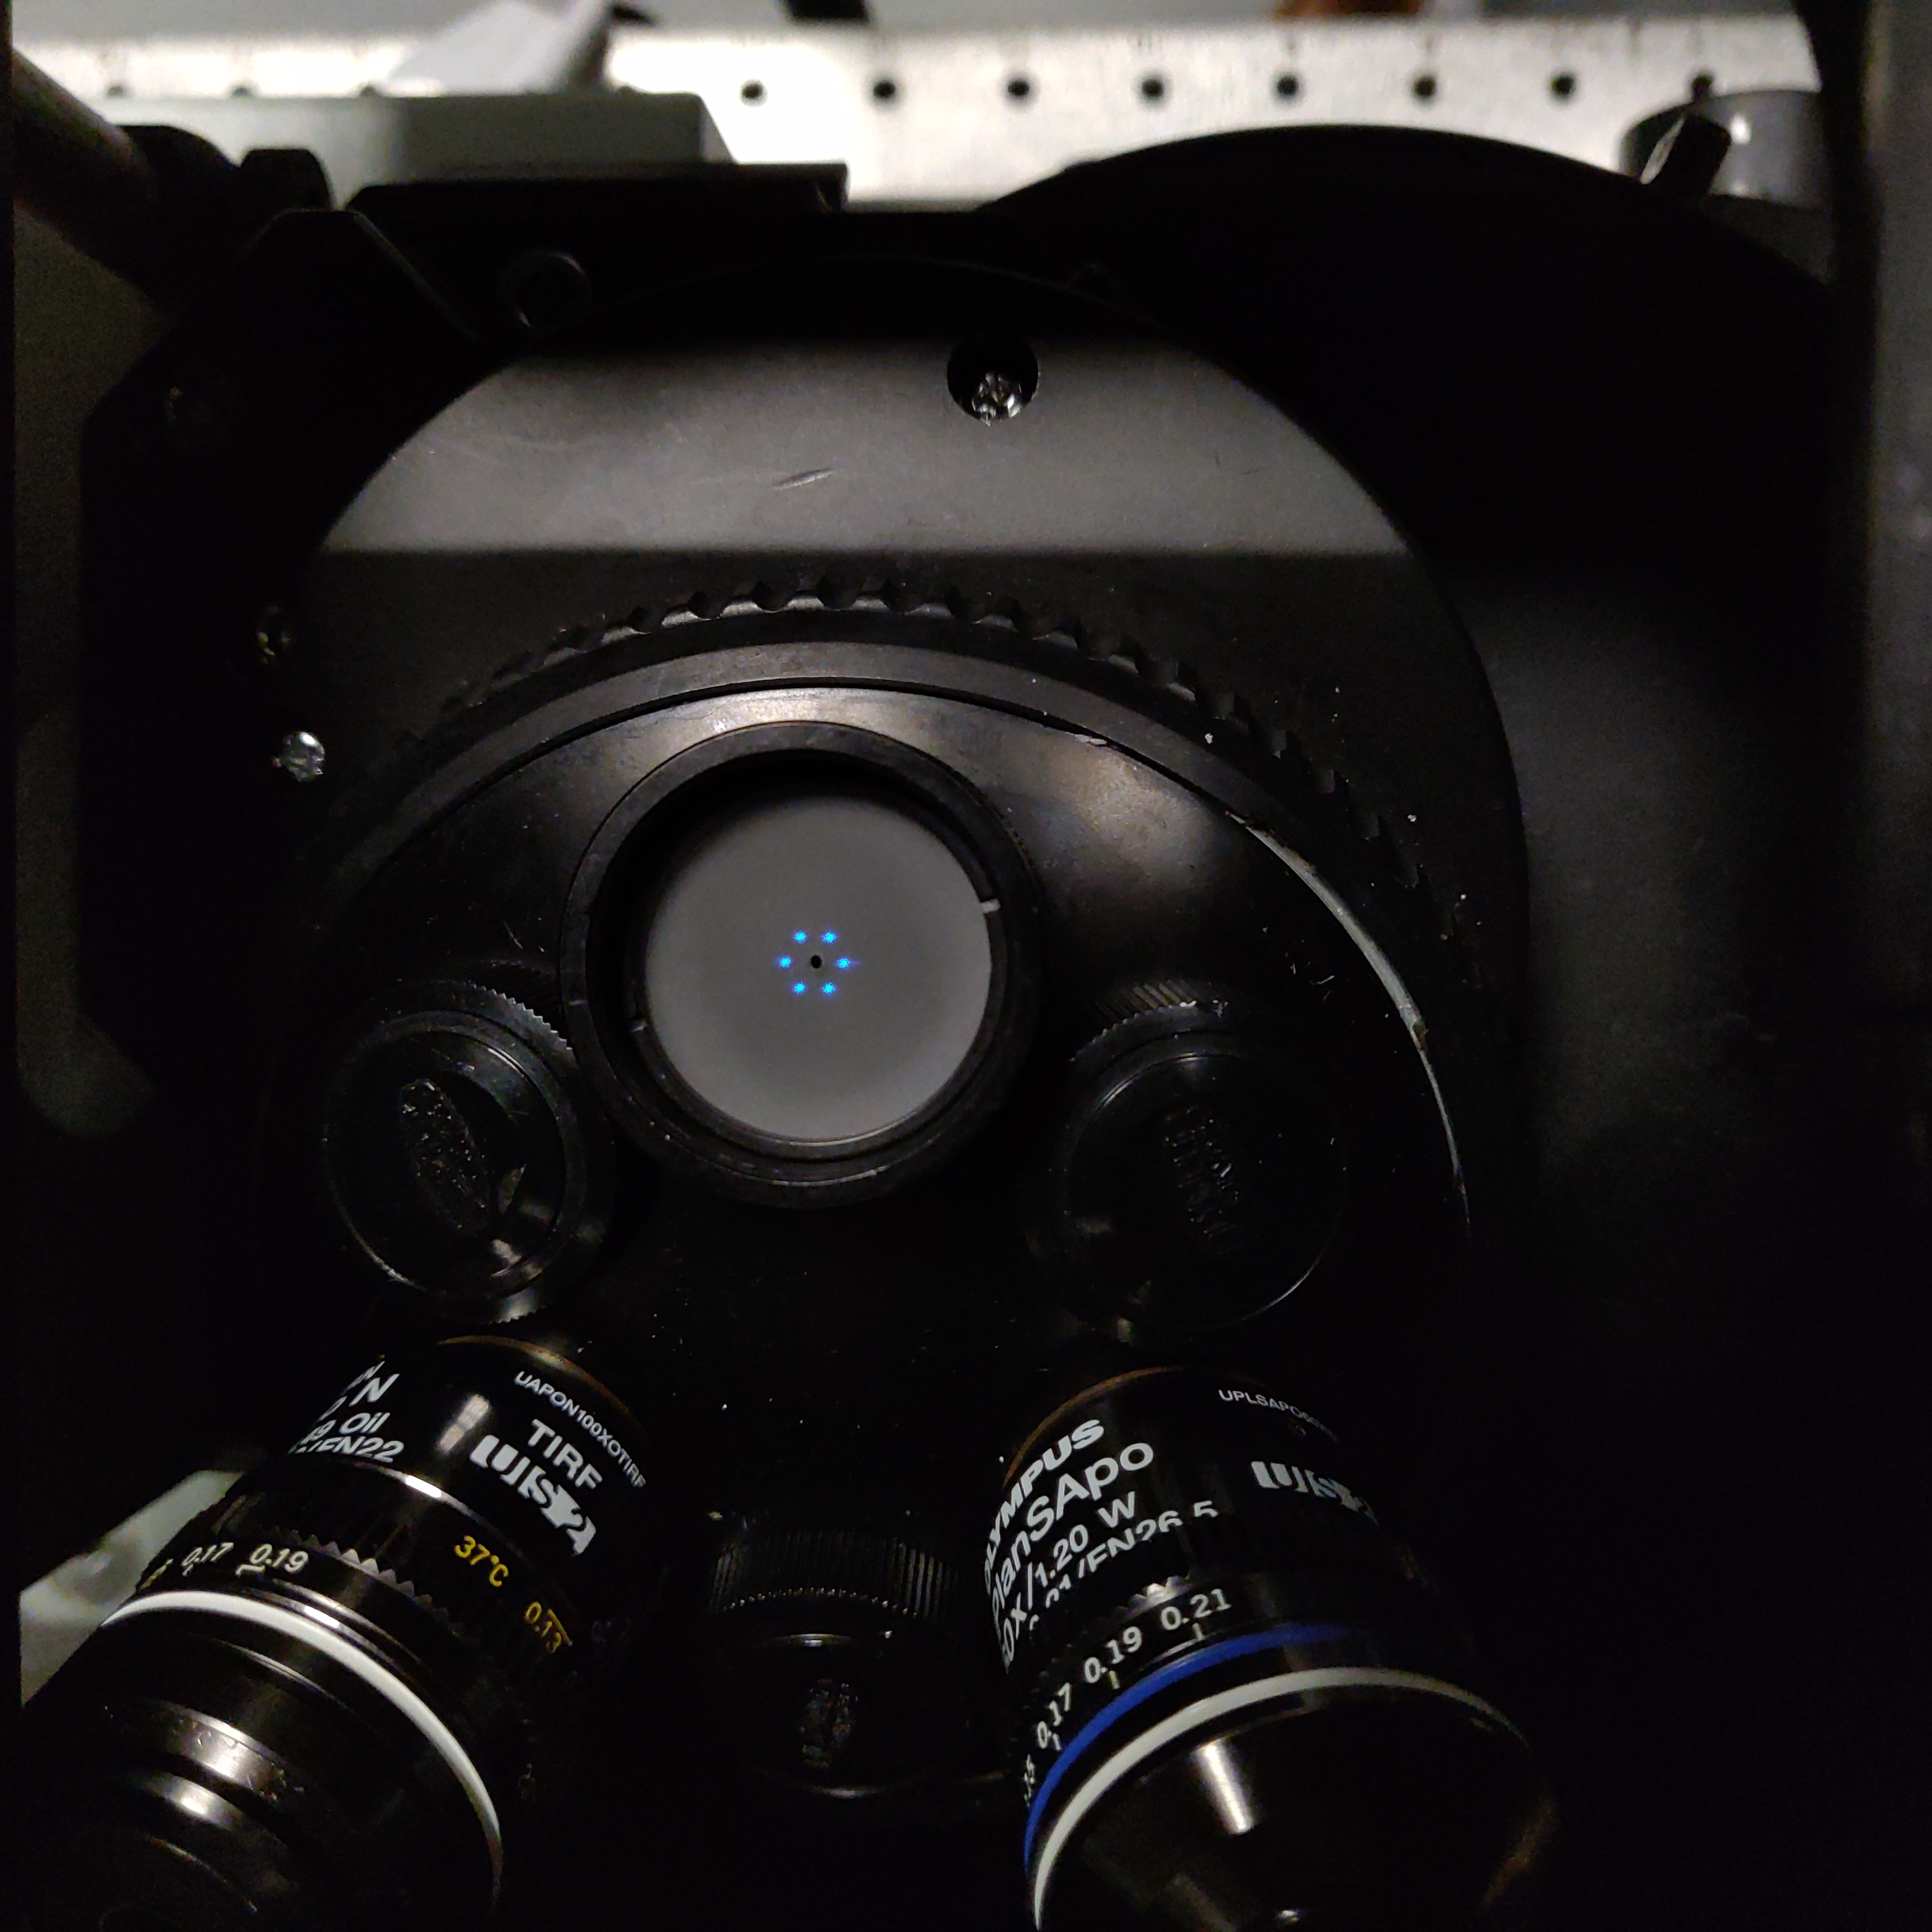
\includegraphics[angle=-90, width=0.6\textwidth]{sim-alignment}
\caption[LAG SIM: Displaying specially designed patterns on the SLM assists with alignment of LAG SIM]{The 3 orientations of the SIM pattern are overlaid on the SLM, such that 6 spots are produced in the Fourier plane for alignment. The spots should be aligned such that the pinhole is at the centre of the spots.}
\label{fig:pinhole-alignment}
\end{figure}

Finally, the `Piezo Offset' section adjusts the z-position of the stage for each channel to account for chromatic offset. 
In practice this offset is very small, on the order of ??\SI{100}{\nano\meter}?? and below the diffraction limit of the microscope. 

\subsection{Log}
The LAG SIM control software logs all activity automatically to Labstep, an online laboratory management system. 

When a user opens the LAG SIM software, they will be asked to enter their name for the online logbook. 
When they press \texttt{Start}, the software sends an HTTP request to a Labstep timeline recording the user's name and the start time. 
Similarly, when the \texttt{Stop \& Close} the software, their name and finish time is logged to the timeline, along with any errors generated by the software during their use. 

Furthermore, every acquisition is also logged to the timeline. 
This contains metadata relating to the acquisition, for example number of t-frames, z-steps, laser powers, and exposure times. 
This is especially helpful is the user is later unsure what acquisition parameters were used for a particular image. 

The user can also add a customised post to the logbook, for example to record an error with the software. 
The online Labstep logbook can be opened by clicking the \texttt{Open logbook} button, opening the webpage shown in Figure~\ref{fig:labstepTimeline}. 

\begin{figure}[htbp!]
\centering
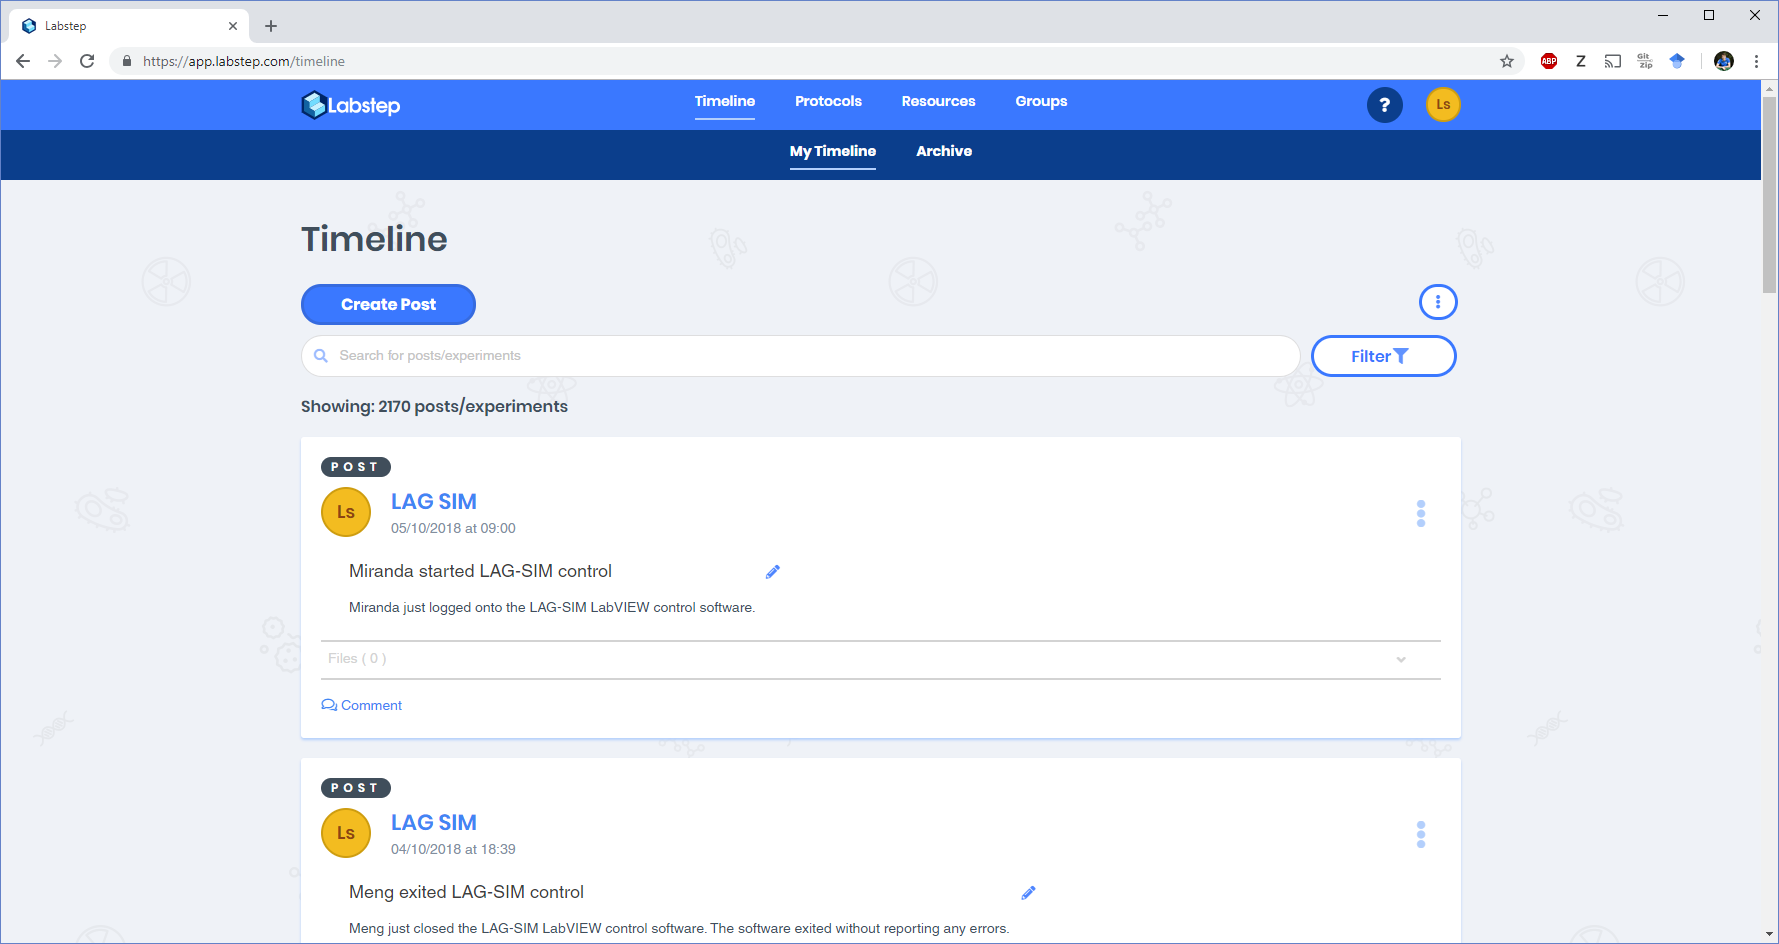
\includegraphics[width=1.0\textwidth]{labstep-timeline}
\caption[LAG SIM: Logging user activity with Labstep allows any problems to be identified and fixed quickly]{User activity is automatically logged to an online logbook hosted on Labstep to identify and fix any problems quickly. This figure shows Miranda logged onto the SIM at 09:00, acquired 2 images, then logged off.} % oops, haven't got her logging off or acquiring 2 images!!! 
\label{fig:labstepTimeline}
\end{figure}

Online logging benefits both the microscope user and the developer, allowing problems to be identified and fixed promptly. 


\section{Reconstruction Algorithms} \label{sec:recon}
Once SIM data is collected, it requires reconstruction to either enhance the resolution, remove out-of-focus light, or a mixture of both.

A basic SIM reconstruction algorithm implements the following steps:
\begin{enumerate}
	\item Extract pattern parameters (orientation angle and phase shift)
	\item Separate Fourier space images into frequency components
	\item \label{step:filterPreShift}Weight components in Fourier space by OTF and filter for noise removal
	\item \label{step:shiftComponents}Shift frequency components into correct position in Fourier space
	\item Inverse Fourier transform for reconstructed image
\end{enumerate}

Additional steps are often added into the basic algorithm to reduce artefacts overall. 
Raw images may be corrected for consistent intensity and contrast across the dataset, and an additional filtering step for noise removal can be applied before the images are separated in Fourier space. 
Note also that step \ref{step:filterPreShift} can be performed after step \ref{step:shiftComponents}, but this can lead to additional artefacts in the reconstructed image. 
Artefacts can furthermore be suppressed by apodisation before the final inverse Fourier transform. 

This basic algorithm will provide resolution enhancement, but does not implement optical sectioning for removing out-of-focus light.
This requires an additional attenuation step, applied simultaneously with step \ref{step:filterPreShift}. 

Various implementations of the SIM reconstruction algorithm exist.
During the course of my PhD, I have utilised and modified three different reconstruction algorithms, and written a plugin for FIJI tailored specifically for LAG SIM and detailed in Section~\ref{sec:lagsimFiji}.
Each implementation has its own merits and disadvantages, discussed in the remainder of this section.

\subsection{Lin Shao SIM Reconstruction}
The first implementation of the resolution-enhancing SIM algorithm used in the Laser Analytics Group was provided by Lin Shao, who worked in the early days of SIM with Mats Gustafsson.
It was developed during his time at Janelia Farm Research Campus, under the supervision of Mats and Eric Betzig.
Lin Shao is now at Yale University; although he is contactable, he is not actively maintaining this piece of software.

The program has no graphics user interface, but is called from the command line. 
Since command line calls can be made from most other programming languages, a custom interface was built in MATLAB for passing in reconstruction parameters, and reconstructing more complex datasets such as multi-channel z-stacks. 

The program was not built for widespread distribution, and as such there is no documentation for it. 
Nor is the program publicly available; requests for a copy of the software have to be made directly to Lin Shao. 
This means the software is complicated to use, and has not been tested and verified by the wider community. 

The algorithm does not implement OTF attenuation, which is used for optical sectioning.
This means it cannot remove out-of-focus light, so is not appropriate for reconstructing 3D image stack. 

Lin's algorithm is written in native CUDA code to run on NVidia graphics cards.
This makes reconstruction very fast - around 1 frame per second on a [SIM COMPUTER GRAPHICS CARD]. 
However, native CUDA must be recompiled from source on every new computer it is used on, and furthermore because the software has not been updated, it does not work with the latest version of CUDA. 
Since Lin's implementation is fast becoming obsolete, it is now only installed on one computer in the Laser Analytics Group, which cannot have graphics updates installed. 

\subsection{SROS-SIM}
Developed by Florian Str\"ohl in the Laser Analytics Group shortly before I arrived, the SROS-SIM program implements both optical sectioning and resolution enhancement. 

SROS-SIM is a MATLAB implementation of the Super Resolution Optical Sectioning algorithm detailed by O'Holleran and Shaw in 2014 [cite]. 
Optical sectioning removes out-of-focus light, so that 3D images can be reconstructed, for example of a whole cell with mitochondria labelled. % Like in Figure ?? 

As a set of MATLAB script and functions, the code can be executed on any computer with a MATLAB license.
Therefore the implementation is available for all major desktop operating systems, and furthermore is easy to modify.
Indeed, I have made modifications to the original code to perform operations on the GPU, bringing a 20X increase in reconstruction speed. 
% Want to show a table of this??

SROS-SIM has the disadvantage of not being publicly available or published and verified by the community. % We think it's got some bugs? 
Furthermore the need for an expensive MATLAB license limits who can use the software. 
Finally, the important step of detecting the illumination pattern parameters is not fully automated, so that the software always requires some user input can cannot be fully automated for a batch reconstruction task.

\subsection{fairSIM}
Developed by Marcel M\"uller and recently published in Nature Methods, fairSIM is an open-source plugin for ImageJ/FIJI, a popular image analysis suite which is also open source and free~\cite{muller2016open}. 
The software is well-documented and hosted on Github, so is continually updated and improved by the community. 

As a reconstruction algorithm, fairSIM implements resolution enhancement and optical sectioning, with two different noise filters. 
It provides the user with complete control over the input parameters, and with debugging options enabled will show detailed visual output at each stage of the reconstruction. 
Although the number of options can be overwhelming for some users, it is powerful and useful software for advanced SIM users. 

The major downfall of fairSIM is the user interface. 
Reconstruction can only be performed on a single-colour, single-frame SIM image. 
This process requires around 20 clicks, and input parameters must be resubmitted for every reconstruction. 
This, coupled with the fact that fairSIM does not have GPU support, makes reconstruction very slow, especially for large, multi-colour image sets. 

% Hessian SIM? 

\subsection{LAG SIM}
LAG SIM is my personal implementation of the SIM reconstruction algorithm, built using the well-documented fairSIM Java library. 
It is designed specifically for the Laser Analytic Group's SIM, simplifying the interface for non-advanced users, and implements a unique parameter-finding technique.

It is available publicly as an ImageJ/FIJI plugin.
This means that it is free, open source, and stays up-to-date for all users. 

The next section describes the LAG SIM plugin in detail, which provides a valuable resource to anyone reconstructing LAG SIM data in the future.

\section{Reconstruction with LAG SIM} \label{sec:lagsimFiji}
Setting SIM reconstruction parameters, particularly for noise filtering and optical sectioning, can be something of a black art.
In LAG SIM, building on the fairSIM plugin, there is a choice of 2 filters, which can be used in combination, 2 filter parameters, 2 apodisation parameters, and 2 attenuation parameters, making a high-dimensional parameter space to optimise over. 
Selecting appropriate values for these parameters requires understanding of what each is for; setting optimum values requires experience and expert skill.

LAG SIM provides a number of user interfaces to assist with parameter optimisation, as well as a number of other tools for batch reconstruction and quick pseudo-widefield previews of the data. 
The main interfaces are shown in Figure~\ref{fig:lagsim-fiji-interface}. 

\begin{figure}[htbp!]
	\centering
		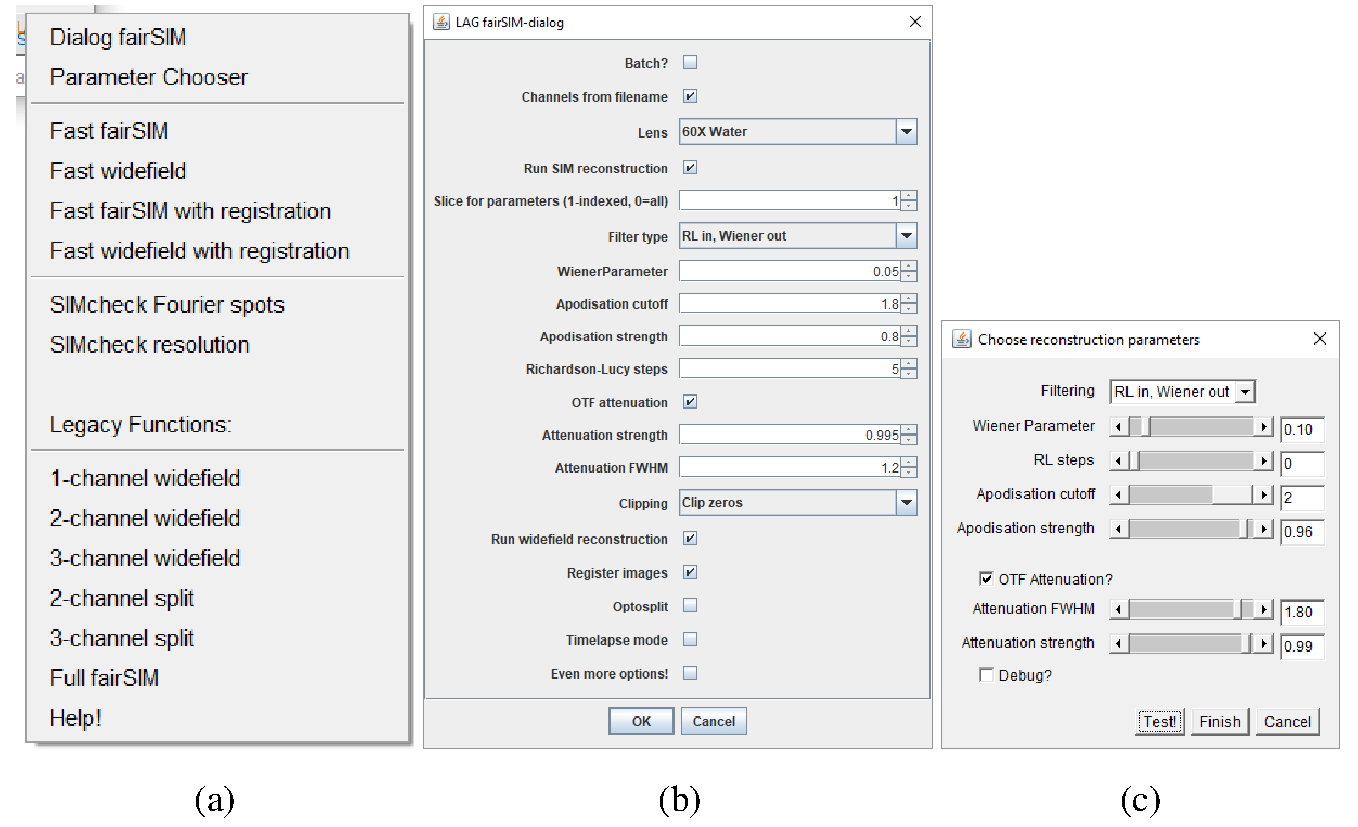
\includegraphics[width=1.0\textwidth]{lagsim-fiji}	
	\caption[LAG SIM: A Fiji interface makes artefact-free reconstruction quick and simple for non-expert users]{The LAG SIM FIJI/ImageJ user interface, utilising the fairSIM reconstruction algorithm, is specifically designed for the LAG SIM to make artefact-free reconstruction quick and straightforward. (a) shows the main LAG SIM menu, with the many reconstruction and SIMcheck tools created; (b) shows the main reconstruction interface, facilitating batch reconstruction; and (c) shows the quick parameter tester, for finding the optimal reconstruction parameters. } % I guess these should be separate figures then. 
\label{fig:lagsim-fiji-interface}
\end{figure}

This section contains an explanation of each parameter, and finishes with a workflow for choosing optimal parameters.
I hope that this provides a useful resource for anyone reconstructing images from the LAG SIM.

\subsection{Illumination detection}
In order to produce an artefact-free reconstruction, the SIM algorithm requires measurement of the illumination pattern to a sub-pixel accuracy. 
This is necessary for correctly performing the Fourier-space shift. 

The LAG SIM reconstruction interface (Figure~\ref{fig:lagsim-fiji-main-interface}) allows the user to choose which slice the illumination pattern is measured from. 
For z-stacks, it is best that the most in-focus slice is used, to get the most accurate measurement. 
Conversely, for a time-series it is best that slice 1 is used, since it will have the least amount of photobleaching. 

Illumination detection with LAG SIM has been designed to require the least amount of user input necessary. 
The user simply needs to select the objective lens used, and the software will infer the necessary information such as pixel size and numerical aperture. 
Wavelength can be extracted directly from the filename if the file is saved using the correct naming convention. 

% Does not provide any feedback to the user about how well the fit went.. 

\subsection{Wiener filter and apodisation}
When the Wiener filtering scheme is used for noise removal, the Wiener parameter and apodisation parameters are used in a complementary fashion. 

Noise filtering is particularly important in SIM due to the non-conventional relationship between signal-to-noise ratio and spatial frequency, caused by Fourier-space shifting. 
A conventional 2D microscope OTF has a peak at 0, and decreases symmetrically, as shown in Figure [?]. 
As noise is assumed to be constant over all spatial frequencies, this causes a decrease in signal-to-noise ratio at high spatial frequencies. 
In SIM, a super-resolution image is built up by shifting the OTF in Fourier space. 
This results in a local maxima in signal-to-noise ratio, as shown in Figure [?]. 
The extra noise in this region causes swirling hexagonal noise patterns, seen in Figure [?]. 

Whilst these patterns are simply how noise looks in a SIM image, they can easily be misinterpreted as features. 
The Wiener filter is a conventional noise filter used in image processing, which successfully removes hexagonal SIM noise as shown in Figure [?]. 
The `Wiener parameter' input is able to control how much noise filtering is applied, as demonstrated by Figures [?]. 

Aggressive noise removal, using high values for the Wiener parameter, is not without consequence. 
Figure [?] shows that as the Wiener parameter is increased, the OTF of the reconstruction becomes less physical. % Not really. 
This results in ringing and negative pixel values around real features in the reconstructed image, seen in Figure [?].  % Somehow need to mention Lucosz in this paragraph? Or "compare to the OTFs in Figures ??" 

\begin{figure}[p]
\centering
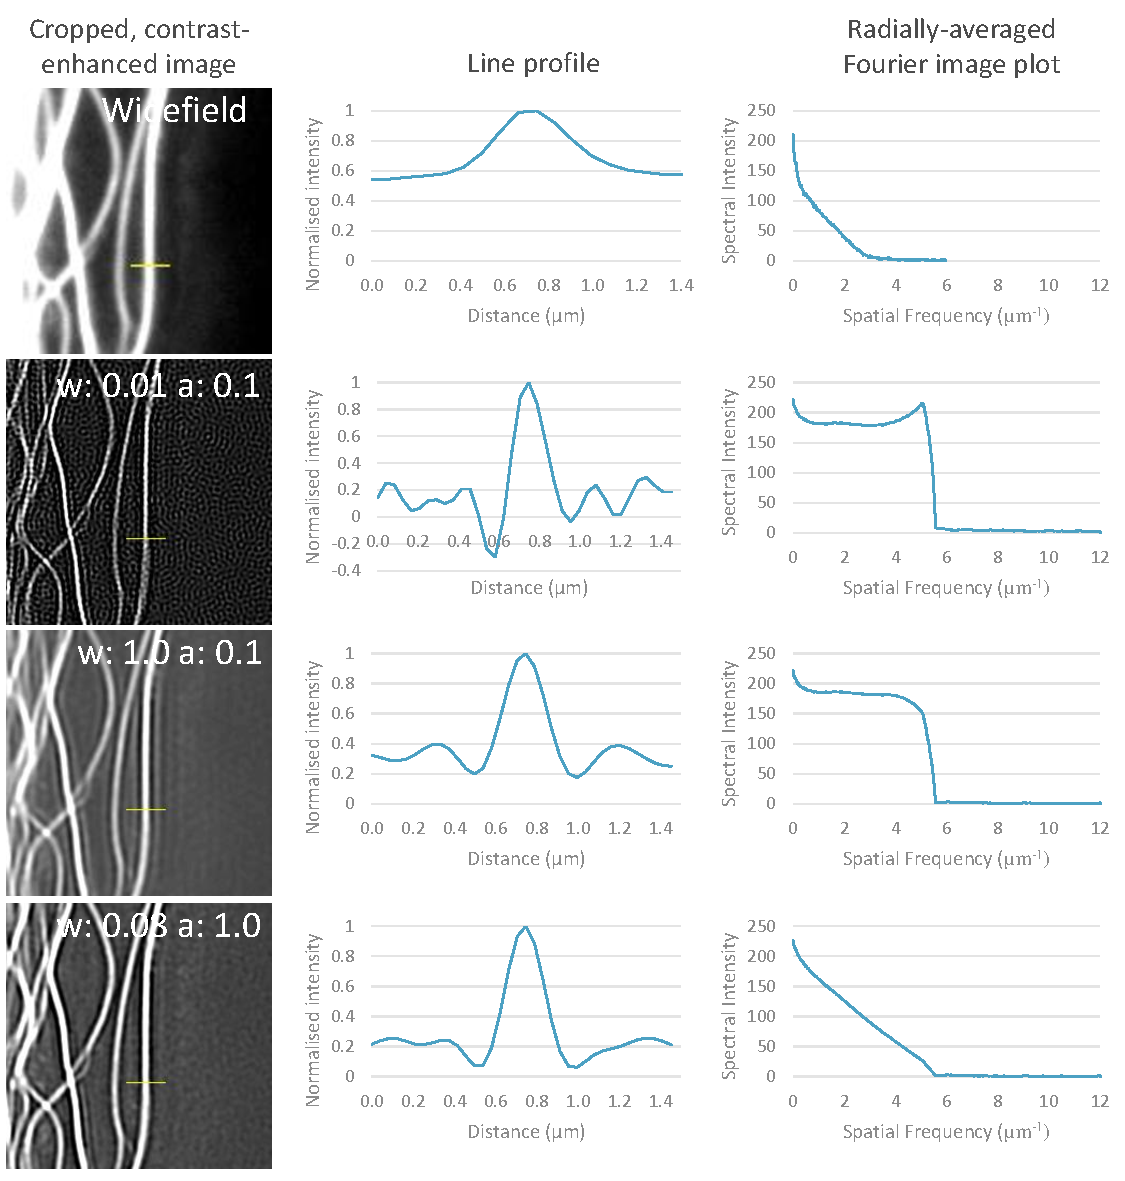
\includegraphics[width=1.0\textwidth]{wiener-parameter}
\caption[LAG SIM: The Wiener parameter and apodisation strength must be chosen to minimise artefacts]{The left column shows crops from a SIM reconstruction with various values of Wiener parameter (w) and apodisation strength (a), and a widefield image for comparison. Note that image contrast has been greatly enhanced to observe the noise pattern. The middle column shows the line profile through a tubule, showing the noise pattern with a low Wiener parameter, ringing with a high Wiener parameter, and suppression of noise and ringing using apodisation. The right hand column shows the radially averaged Fourier transform plot of each image; note the local peak when a low Wiener filter is used, which boosts noise at this frequency causing the unconventional noise pattern.}
% Really need to add a, b, c, etc to this, I think. 
\label{fig:wiener-parameter}
\end{figure}

To reduce ringing artefacts, the reconstructed image is passed through an apodisation filter. 

Apodisation is a type of low-pass filter, reducing power in higher spatial frequencies. 
The radius of the apodising filter in Fourier space is controlled by the `apodisation cutoff' parameter, where a value of 1 corresponds to the cutoff spatial frequency of the objective lens based on its numerical aperture and the emission wavelength of the image. 
The shape of the apodisation filter is controlled by the `apodisation strength' parameter, where a value of 0 gives a tophat filter, $\frac{1}{\sqrt{2}}$ a triangular filter, and larger values reduce the full-width half maximum. % As shown in figure? 

The apodisation cutoff should be as large as possible, with a maximum value of 2 for full SIM resolution enhancement. 
Smaller cutoff values reduce the radius of the reconstruction in Fourier space, directly reducing resolution; a value of 1 corresponds to widefield resolution. 
Furthermore, the apodisation strength should be as small as possible whilst still removing ringing artefacts for maximum resolution. 

\subsection{Richardson-Lucy Filtering}
An alternative filtering scheme for noise removal is the Richardson-Lucy deconvolution. 
The Richardson-Lucy filtering scheme has several advantages over Wiener filtering: it guarantees non-negative pixel values, removing the need for an apodisation step; it does not cause ringing in the reconstructed image; and it only takes one parameter LAG SIM.

% see Perez, Change, Stelzer Scientific reports 2016

\begin{figure}[p]
\centering
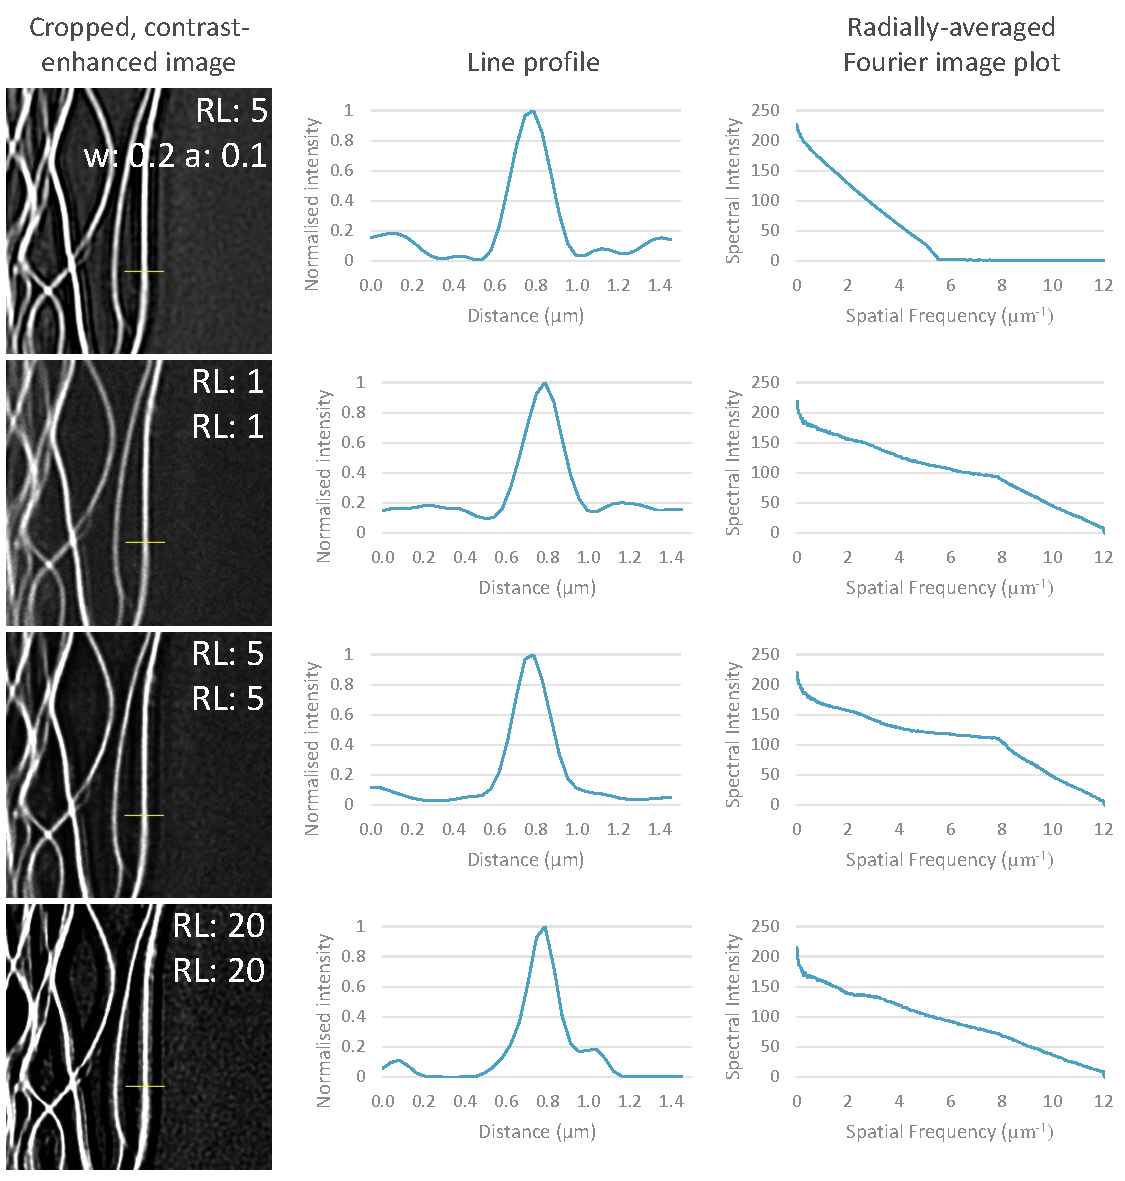
\includegraphics[width=1.0\textwidth]{rl-filtering-figure}
\caption[LAG SIM: Richardson-Lucy filtering can further reduce SIM reconstruction artefacts]{Richardson-Lucy deconvolution on the raw data reduces noise, leading to fewer artefacts in the Weiner-filter reconstruction. Furthermore using Richardson-Lucy filtering for reconstruction produces a more conventionally shaped OTF than Wiener filtering, which further reduces the number of reconstruction artefacts.}
\label{fig:rl-filtering}
\end{figure}

% Who first suggested its use on SIM images? 
Richardson-Lucy deconvolution is an iterative process, where each iteration of the algorithm converges on the maximum likelihood solution of an image corrupted with Poisson noise. 
The number of iterations is set in LAG SIM by the user.
More iterations leads to a thinner point spread function, and thus higher perceived resolution, but also leads to noise amplification, which can cause a speckle pattern to appear in the reconstructed image. % Should probably have a figure of this. 

This filtering scheme can be used on the final reconstructed image in place of Wiener filtering. 
It can also be used on the raw data set before reconstruction, reducing noise at the start of the algorithm. 
Pre-filtering is especially effective at removing the strange SIM speckle, since less noise is shifted and boosted in Fourier space. % Figure above. Because these things end up looking really good. 

Richardson-Lucy input filtering can be used in combination with either the Wiener filter or with more Richardson-Lucy filtering on the reconstructed image. 
Therefore there are in total 4 filtering schemes offered by LAG SIM: Wiener-output; RL-output; RL-input, Wiener-output; and RL-input, RL-output. 

\subsection{OTF Attenuation}
In conventional widefield microscopy, light from areas above and below the focal plane are captured by the lens, causing out-of-focus light and effectively reducing the axial resolution of the microscope. 
When observing the 3D widefield OTF, it is obvious that this is the case. 
The OTF has no support in the axial direction at low frequencies, which is known as the `missing cone' problem. 

In the Laser Analytics Group's SIM setup, the illumination pattern is only projected onto the sample plane; therefore out of focus light does not show the SIM pattern.
Intuitively, one would think this out-of-focus light can be removed by rejecting any part of the image that does not have the SIM pattern, and only showing the in-focus parts of the image with SIM pattern on them. 
O'Holleran and Shaw show that this is achieved practically by attenuating certain parts of the OTF during reconstruction. [cite]

If the center part of the OTF is computationally removed, out-of-focus light will be removed from the reconstructed image.
In conventional widefield microscopy, this would have the side-effect of also removing low-frequency information from the image. 
In structured illumination microscopy, however, this information can be recovered from shifted components in Fourier space. 

\begin{figure}[htbp!]
\centering
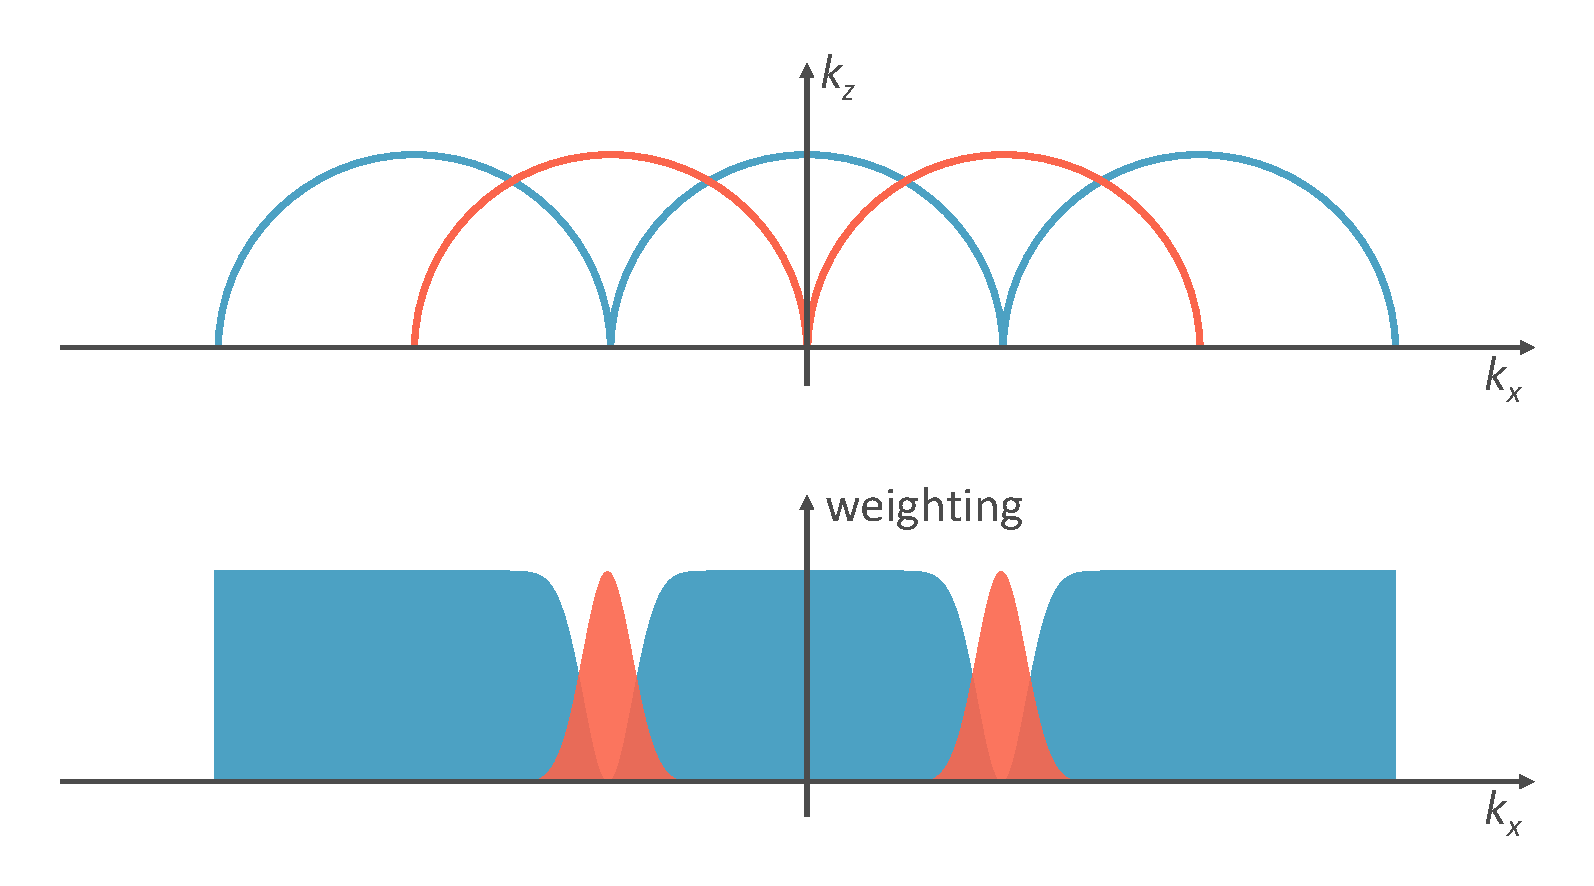
\includegraphics[width=1.0\textwidth]{oholleran-otf-attenuation}
\caption[LAG SIM: OTF attenuation]{By suppressing the OTF in areas where it does not have axial support, out-of-focus light is removed. The in-focus light at these spatial frequencies can still be reconstructed as a result of the shifted OTF from SIM reconstruction. Adapted from~\cite{oholleran2014optimized}. }
\label{fig:oholleran-otf}
\end{figure}

Figure~\ref{fig:oholleran-otf}, reproduced from [cite?], shows which parts of the OTF should be attenuated to achieve optical sectioning with no loss of resolution. 
The optical sectioning is controlled by a Gaussian notch in the first-order passbands, and a complementary Gaussian in the zero-order passband. 
The width and depth of this passband is controlled in LAG SIM with the parameters `Attenuation FWHM' and `Attenuation strength' respectively.

% Does optical sectioning in this way sacrafice resolution? I don't think so? 

Note that OTF attenuation cannot be used with the Richardson-Lucy output filter. 
% maybe this isn't true in the latest version? Need to play about a bit more in Fourier space. 

The water lens is set up for optical sectioning. 

Out-of-focus light makes creating 3D reconstructions impossible, as shown in Figure ?. % 3D reconstruction figure
Using optical sectioning to remove this light allows 3D reconstructions of the sample to be created, which can reveal information otherwise unobservable, such as whether a particle is located on the inside or outside of a cell membrane. 

\section{Results and Discussion: SIM showcase} \label{sec:sim-showcase}
LAG SIM has been designed to be a versatile and user-friendly microscope, providing high-speed multi-colour imaging surpassing the diffraction limit with optical sectioning provided computationally or with TIRF. 
With a number of useful automations, LAG SIM can be used to create timelapse videos, 3D reconstructions, large mosaic images, and for unsupervised imaging of multiple cells at different locations around the coverslip. 
As a result, the microscope can and has found applications in a wide variety of biological investigations.

This section presents a small selection of experiments utilising a range of LAG SIM's capabilities. 
Acquisition and reconstruction methods are provided as a resource for researchers interested in conduction similar experiments with the microscope. 

\subsection{Bead alignment slide}
For any multicolour SIM experiments, a slide of multicolour subdiffraction beads can be used for measuring and correcting chromatic offset, and allows aberrations to be minimised. 

If an appropriate slide is not available, one can be produced as follows: 
\begin{enumerate}
	\item Sonicate \SI{0.1}{\micro\metre} beads for \SI{10}{\minute}
	\item Dilute beads 1:10 in distilled water, producing a suspension of density [?? ]
	\item Dispense \SI{20}{\micro\litre} of the diluted beads onto a coverglass, or \SI{50}{\micro\litre} into an 8-well Labtek
	\item Wait for the solution to dry, about \SI{2}{\hour}
	\item Add mounting medium: immersion oil for use with the 100$\times$ oil lens, or water for use with the 60$\times$ water lens. 
	\item Mount the coverglass on a glass slide, or replace the lid on the Labtek and seal with Parafilm to prevent spillages
\end{enumerate}

\begin{figure}[p]
\centering
\begin{subfigure}[b]{0.49\textwidth}
	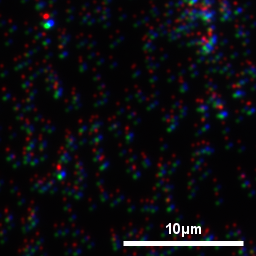
\includegraphics[width=\textwidth]{recon-beads-unaligned}
	\caption{}\label{fig:recon-beads-unaligned}
\end{subfigure}
\hfill
\begin{subfigure}[b]{0.49\textwidth}
	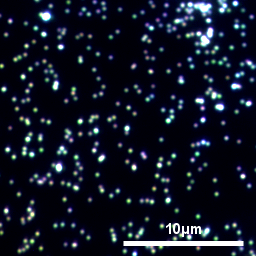
\includegraphics[width=\textwidth]{recon-beads-registered}
	\caption{}\label{fig:recon-beads-registered}
\end{subfigure}
\caption[LAG SIM: Multicolour alignment beads are used for correcting chromatic offset]{A small chromatic offset between the three SIM colour channels can be seen in (a). When the offset is corrected, as in (b), the beads appear white; the offset parameters can then be used to correct other multi-colour images captured during the same imaging session.  } 
\label{fig:recon-beads}
\end{figure}

When the beads slide is viewed on the microscope, aberrations can be minimised by adjusting the correction collar on the objective lens and observing the point-spread function of individual beads. 
For minimal aberrations, the point-spread function should be symmetrical when defocussing above and below the bead layer. 

To measure chromatic offset, a mutli-colour acquisition should be performed with the same settings as the subsequent biological experiment. 
Reconstruction in LAG SIM for Fiji should then be performed with the following suggested parameters: \newline
\begin{tabular}{p{0.5\textwidth}}
\begin{labelling}[margin=OTF attenuation]
	\item[Filter] RL in, RL out
	\item[RL steps] 5
	\item[OTF attenuation] false
\end{labelling}
\end{tabular}

After reconstruction, there will be some chromatic offset between each channel, as shown in Figure~\ref{fig: }. 
After registration and correction, an RGB colour map should produce white beads. 

% figure of beads with chromatic offset, then corrected


\subsection{Resolution-enhanced optical sectioning of ?? cells}
A frequent biological application of microscopy is imaging cultured cells under different treatments or with different genetic modifications. 
In this particular application, which is described in greater in Chapter~\ref{chap:MOF}, we treated the cells with a metal organic framework (MOF) as a drug delivery system. 
The goal was to observe uptake of the drug into live cells over a period of \SI{24}{\hour}. 

The MOF was naturally fluorescent in the \SI{488}{\nano\metre} excitation channel. 
Endosomes were labelled with [?? early endosome stain], and the nucleus was labelled with [?? si dna stain] to visualise the cell. 

To ensure MOF had entered the cell, rather than sitting on the cell membrane, it was necessary to view the cells in 3D. 
The 60$\times$ water lens was selected, and operated optical sectioning SIM mode. 
A z-stack of 3-colour SIM images was captured using the filter wheel, with a z-step of \SI{0.2}{\micro\metre} between each plane. 
Since fast dynamics were not observed, a \SI{200}{\milli\second} exposure time was used per raw frame, to ensure a high signal-to-noise ratio. 

The z-stack was reconstructed by utilising OTF attenuation for optical sectioning. 
The following parameters were used for the LAG SIM Fiji plugin:\newline
\begin{tabular}{p{0.5\textwidth}p{0.5\textwidth}}
\begin{labelling}[margin={Attenuation strength}]
	\item[Filter] RL in, Wiener out
	\item[Wiener parameter] 0.05
	\item[Apodiation cutoff] 1.7
	\item[Apodiation strength] 0.8
\end{labelling} &
\begin{labelling}[margin={Attenuation strength}]
	\item[RL steps] 5
	\item[OTF attenuation] true
	\item[Attenuation FWHM] 1.2
	\item[Attenuation strength] 0.995 
\end{labelling} % NEED TO CHECK THESE!!!
\end{tabular}

Images were captured at time points of \SI{30}{\minute}, \SI{1}{\hour}, \SI{2}{\hour}, \SI{6}{\hour}, \SI{8}{\hour} and \SI{24}{\hour} after application of the MOF, to observe that the cells were indeed able to take up MOF.
Although an Okolab incubation stage was used to maintain a \SI{5}{\percent} CO\textsubscript{2}, \SI{37}{\degreeCelsius} environment for the cells, they did not survive on the microscope stage over the full \SI{24}{\hour} period, so were returned to the lab incubator between imaging; therefore, different cells were imaged at each time point. 
A 3D reconstruction is shown in Figure~\ref{fig:recon-mofcell}. 

\begin{figure}[tbp!]
\centering
\begin{subfigure}[b]{0.7\textwidth}
	\includegraphics[width=\textwidth]{recon-mofcell-2D}
	\caption{}\label{fig:recon-mofcell-2D}
\end{subfigure}

~\newline
\begin{subfigure}[b]{0.7\textwidth}
	\includegraphics[width=\textwidth]{recon-mofcell-3D}
	\caption{}\label{fig:recon-mofcell-3D}
\end{subfigure}
\caption[LAG SIM: 3D reconstruction of ?? cell]{3 colour MOF in cell in 3D. Scalebar in (a) is \SI{20}{\micro\metre}}
\label{fig:recon-mofcell}
\end{figure}

\subsection{Fast, multicolour imaging of dynamics in ?Meng's cells}
During experiments on the dynamics of endoplasmic reticulum (ER), which are detailed in Chapter~\ref{chap:ER}, we observed a strong interaction between ER and other organelles, including lysosomes and tubulin. 
To develop a deeper understanding of these relationships, we required fast, high-resolution imaging of live cells in multiple colour channels simultaneously. 

For high resolution, the 100$\times$ oil lens was chosen, although, because we were looking deeper than \SI{100}{\nano\metre} into the cell, it was not operated in TIRF mode. 
To facilitate simultaneous multi-colour imaging, the Optosplit was employed. 
Cross-talk between colour channels was minimised by labelling just two organelles per experiment, in the \SI{488}{\nano\metre} and \SI{640}{\nano\metre} excitation channels. 

A time-series of SIM images was acquired at a raw exposure time of SI\SI{10}{\milli\second} per frame. 
These were reconstructed with the following parameters: \newline
\begin{tabular}{p{0.5\textwidth}}
\begin{labelling}[margin=OTF attenuation]
	\item[Filter] RL in, RL out
	\item[RL steps] 5
	\item[OTF attenuation] false
\end{labelling}
\end{tabular}

\begin{figure}[tbp!]
\centering
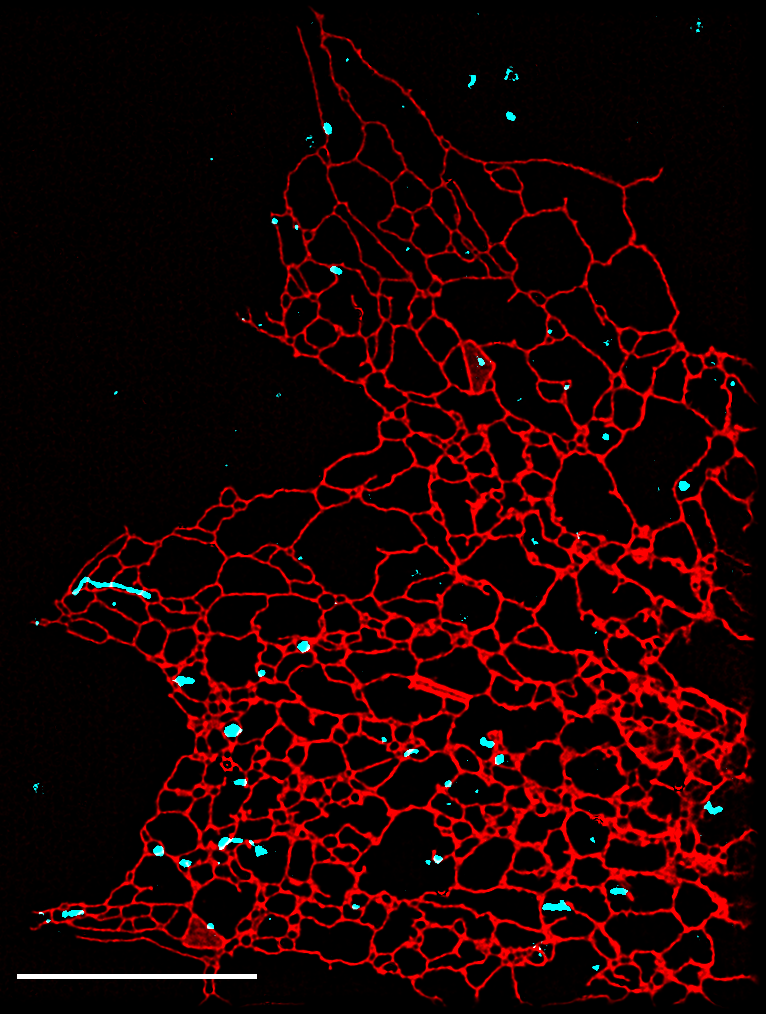
\includegraphics[width=1.0\textwidth]{recon-er-cell}
\caption[LAG SIM: Fast, multi-colour imaging of ER in cells reveals co-localisation between lysosomes and ER tubules]{HEK293 cells with ER is coloured in blue, and lysosomes are coloured in orange. Capturing a timelapse utilising the Optosplit and optical sectioning SIM reveals a strong co-localisation between lysosomes and ER tubules. }
\label{fig:recon-er-cell}
\end{figure}
% Figure, with a description. 
% Hessian SIM as an extra denoising step? 

Work on these observations is ongoing, with a variety of genetic mutations now being applied to cell lines to observe differences in organelle interaction. 


\subsection{Timelapse TIRF imaging of ?Anchal's cell membrane}
Structure on the cell membrane is difficult to observe in epi-fluorescent microscopy due to out-of-focus light obscuring details on the membrane. 
LAG SIM's capability to perform TIRF was therefore vital for imaging actin dynamics on the membrane on ??(COS-7?) cells. 
% Seen in Figure. 

In this experiment, ring structures in the actin were found to colocalise with ??protein. 
By performing time-lapse imaging, and taking a short video every \SI{10}{\minute}, we were able to observe that these ring structures produce projections of actin which spread through the cell. 
The bookmarking feature of LAG SIM was used to record the location of a cells cells distributed across the cover glass, so that many cells could be captured in one imaging session. 

The 100$\times$ oil lens was chosen for its TIRF capabilities. 
2-colour TIRF-SIM imaging was performed sequentially at a frame rate of ??. 
The following parameters were used for reconstruction: \newline
\begin{tabular}{p{0.5\textwidth}}
\begin{labelling}[margin=OTF attenuation]
	\item[Filter] RL in, RL out
	\item[RL steps] 5
	\item[OTF attenuation] false
\end{labelling}
\end{tabular}

The concentration of fluorescent molecules was low to ensure the experiment was as physiologically relevant as possible, so Hessian de-noising was performed in MATLAB after the reconstruction. 

\begin{figure}[tbp!]
\centering
\begin{subfigure}[b]{0.7\textwidth}
	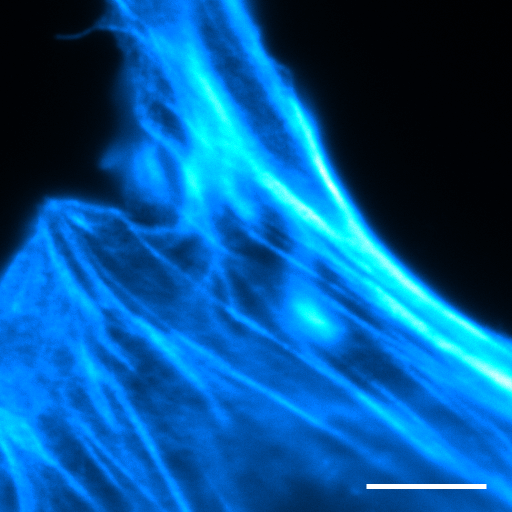
\includegraphics[width=\textwidth]{widefield-actin}
	\caption{}\label{fig:widefield-actin}
\end{subfigure}

~\newline
\begin{subfigure}[b]{0.7\textwidth}
	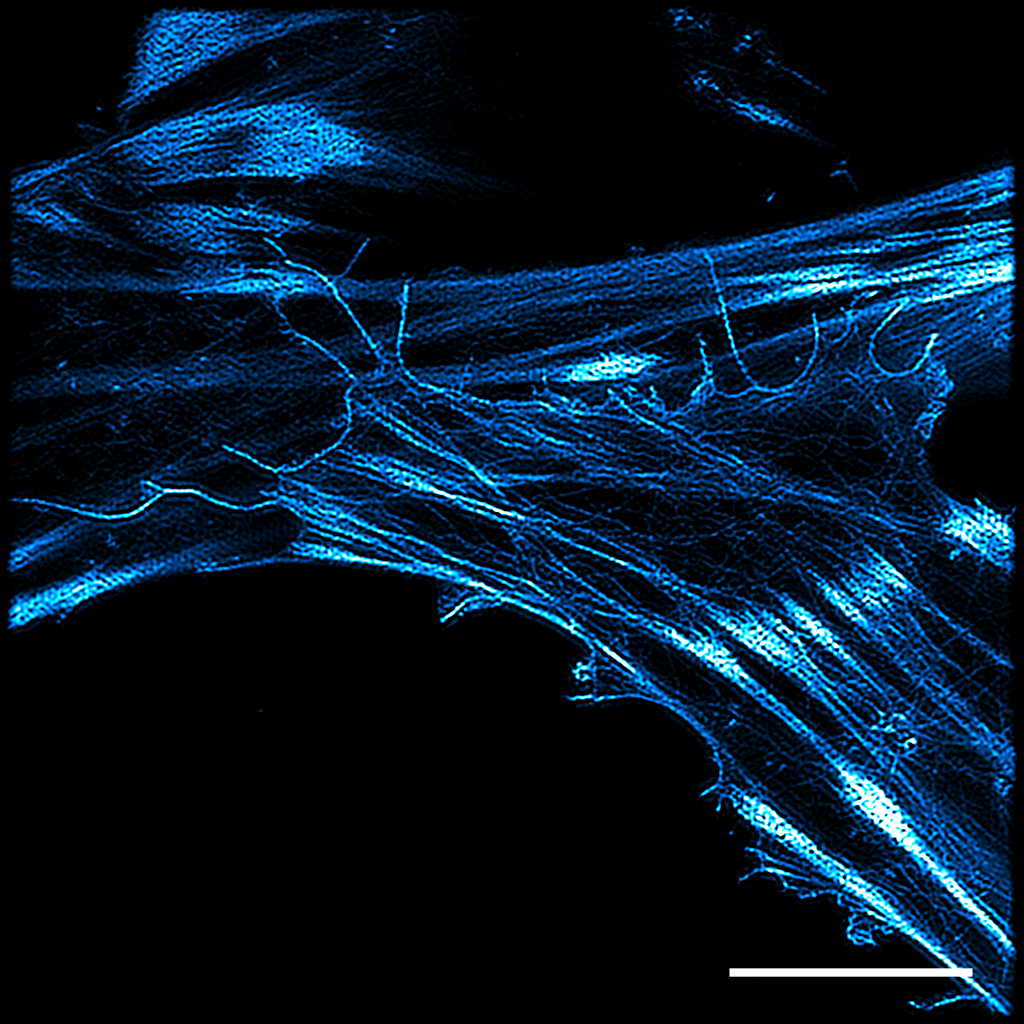
\includegraphics[width=\textwidth]{recon-tirf-actin}
	\caption{}\label{fig:recon-tirf-actin}
\end{subfigure}
\caption[LAG SIM: TIRF imaging of actin in COS-7 cells removes out-of-focus light]{(a) shows actin labelled in COS-7 cells, where out-of-focus light blurs details in the actin. Utilising TIRF-SIM, shown in (b), enhances resolution and removes out-of-focus light. Scalebar is \SI{10}{\micro\metre}. }
\label{fig:recon-actin}
\end{figure}

Further research into these observations is ongoing. 


\subsection{Resolution-enhanced optical sectioning for tissue imaging}
The versatility of LAG SIM also allows it to perform tissue imaging beyond the diffraction limit. 
\SI{8}{\micro\metre}-thin slices of mouse brain were labelled to study the myelin sheath of oligodendrocytes. 
Myelin was labelled in one of two colours, depending on whether the origin of the cell was from the [front or back] of the brain. 
The end of the each myelin sheath was labelled with a 3\textsuperscript{rd} colour to measure the node of Raniver (that is, the gap between two myelin sheaths), to discover whether there is an observable difference between the two oligodendrocyte types related to disease pathology. 

To allow the greatest imaging depth, the lens with the closest refractive index matched to the tissue was chosen; in this case, the 60$\times$ water lens. 
A greater penetration depth could be achieved with a lens better matched to the tissue's refractive index, for example a silicon-oil immersion lens with a refractive index of ???1.4???, if one is available. 
A z-stack was captured with a step-size of \SI{0.2}{\micro\metre}, to build up a 3D image. 
Cells were fixed, so a raw frame exposure time of [???] was used to ensure a high signal-to-noise ratio. 

To reconstruct the slices, the following parameters were used in the LAG SIM Fiji plugin:\newline
\begin{tabular}{p{0.5\textwidth}p{0.5\textwidth}}
\begin{labelling}[margin={Attenuation strength}]
	\item[Filter] RL in, Wiener out
	\item[Wiener parameter] 0.05
	\item[Apodiation cutoff] 1.7
	\item[Apodiation strength] 0.8
\end{labelling} &
\begin{labelling}[margin={Attenuation strength}]
	\item[RL steps] 5
	\item[OTF attenuation] true
	\item[Attenuation FWHM] 1.2
	\item[Attenuation strength] 0.995 
\end{labelling} % NEED TO CHECK THESE!!!
\end{tabular}

Furthermore, the bookmarking function of LAG SIM was used to create a mosaic pattern, allowing reconstruction of a full brain slice in a single tiled image, as shown in Figure~\ref{fig:wholebrain}. 
Although in the end no statistical difference was calculated between the two cell types, this experiment demonstrated LAG SIM's ability to image tissue samples. 

\begin{figure}[tbp!]
\centering
\includegraphics[width=1.0\textwidth]{recon-brain}
\caption[LAG SIM: Multi-colour optical sectioning SIM to measure the node of Raniver]{Oligodendrocytes from the dorsal and ventral region of the brain are coloured in magenta and cyan respectively. The end of the myelin sheath is coloured in orange, and can be used to measure the length of the node of Raniver. Optical sectioning SIM was used on \SI{8}{\micro\metre} brain slices. Scalebar is \SI{10}{\micro\metre}. }
\label{fig:recon-brain}
\end{figure}

\section{Conclusion}
LAG SIM has been restored to its fast imaging speed of 11 super-resolution frames per second through the introduction of a Pockels cell for polarisation rotation. 
The Pockels cell is a robust, future-proof solution to ensure that the SIM illumination is generated with high pattern contrast. 
With this successfully in place, the other desirable features of LAG SIM could be addressed. 

The instrument can now quickly switch between TIRF imaging, resolution-enhanced SIM imaging and SIM optimised for optical sectioning through a combination of well-designed software and straightforward hardware tweaks. 
This makes it suited to a wide variety of biological imaging experiments, as presented in the SIM showcase. 

The addition of an Optosplit, made possible by the implementation of the Pockels cell rather than an LCVR, further enhances LAG SIM's fast imaging capability. 
Rather than requiring the use of a filter wheel to switch between colour channels, 3 colours can be imaged simultaneously. 
This removes any mechanical movement from the system, reducing the fastest 3-channel acquisition from \SI{470}{\milli\second} to the headline \SI{90}{\milli\second}, a five-fold improvement in frame rate. 

Considerable care has been taken to ensure the microscope can be used by non-expert users. 
The interface is clear and compact, and can be taught to new users in a single imaging session. 
This means that LAG SIM can be used unsupervised, saving time and allowing for the microscope to perform a diverse range of world-leading biological research.

Finally, the LAG SIM Fiji plugin complements the easy-to-use microscope to help users generate artefact-free images. 
As shown throughout this chapter, reconstruction is a complicated process involving complex mathematics and optical engineering. 
LAG SIM simplifies this process, so that a user can go from hypothesis to result without the need for a full-time SIM expert. 

In addition to the SIM showcase presented here, Chapters~\ref{chap:MOF} and \ref{chap:ER} detail two successful experiments facilitated by LAG SIM. 
Before that, however, Chapter~\ref{chap:FPB} reveals FPBioimage, a user-friendly tool for visualising and sharing 3D volumetric data, such as those obtained through optical sectioning on the LAG SIM. 